% Generated extraction from local PDFs in docs/完全理解！筱泽广的机器学习$\cdot$数学优化研讨课~第一讲~.
% This is an editable LaTeX fragment, not yet polished as booklet prose.
\chapter*{完全理解！筱泽广的机器学习$\cdot$数学优化研讨课：第一讲}
\addcontentsline{toc}{chapter}{完全理解！筱泽广的机器学习$\cdot$数学优化研讨课：第一讲}
\begin{figure}[p]
\centering
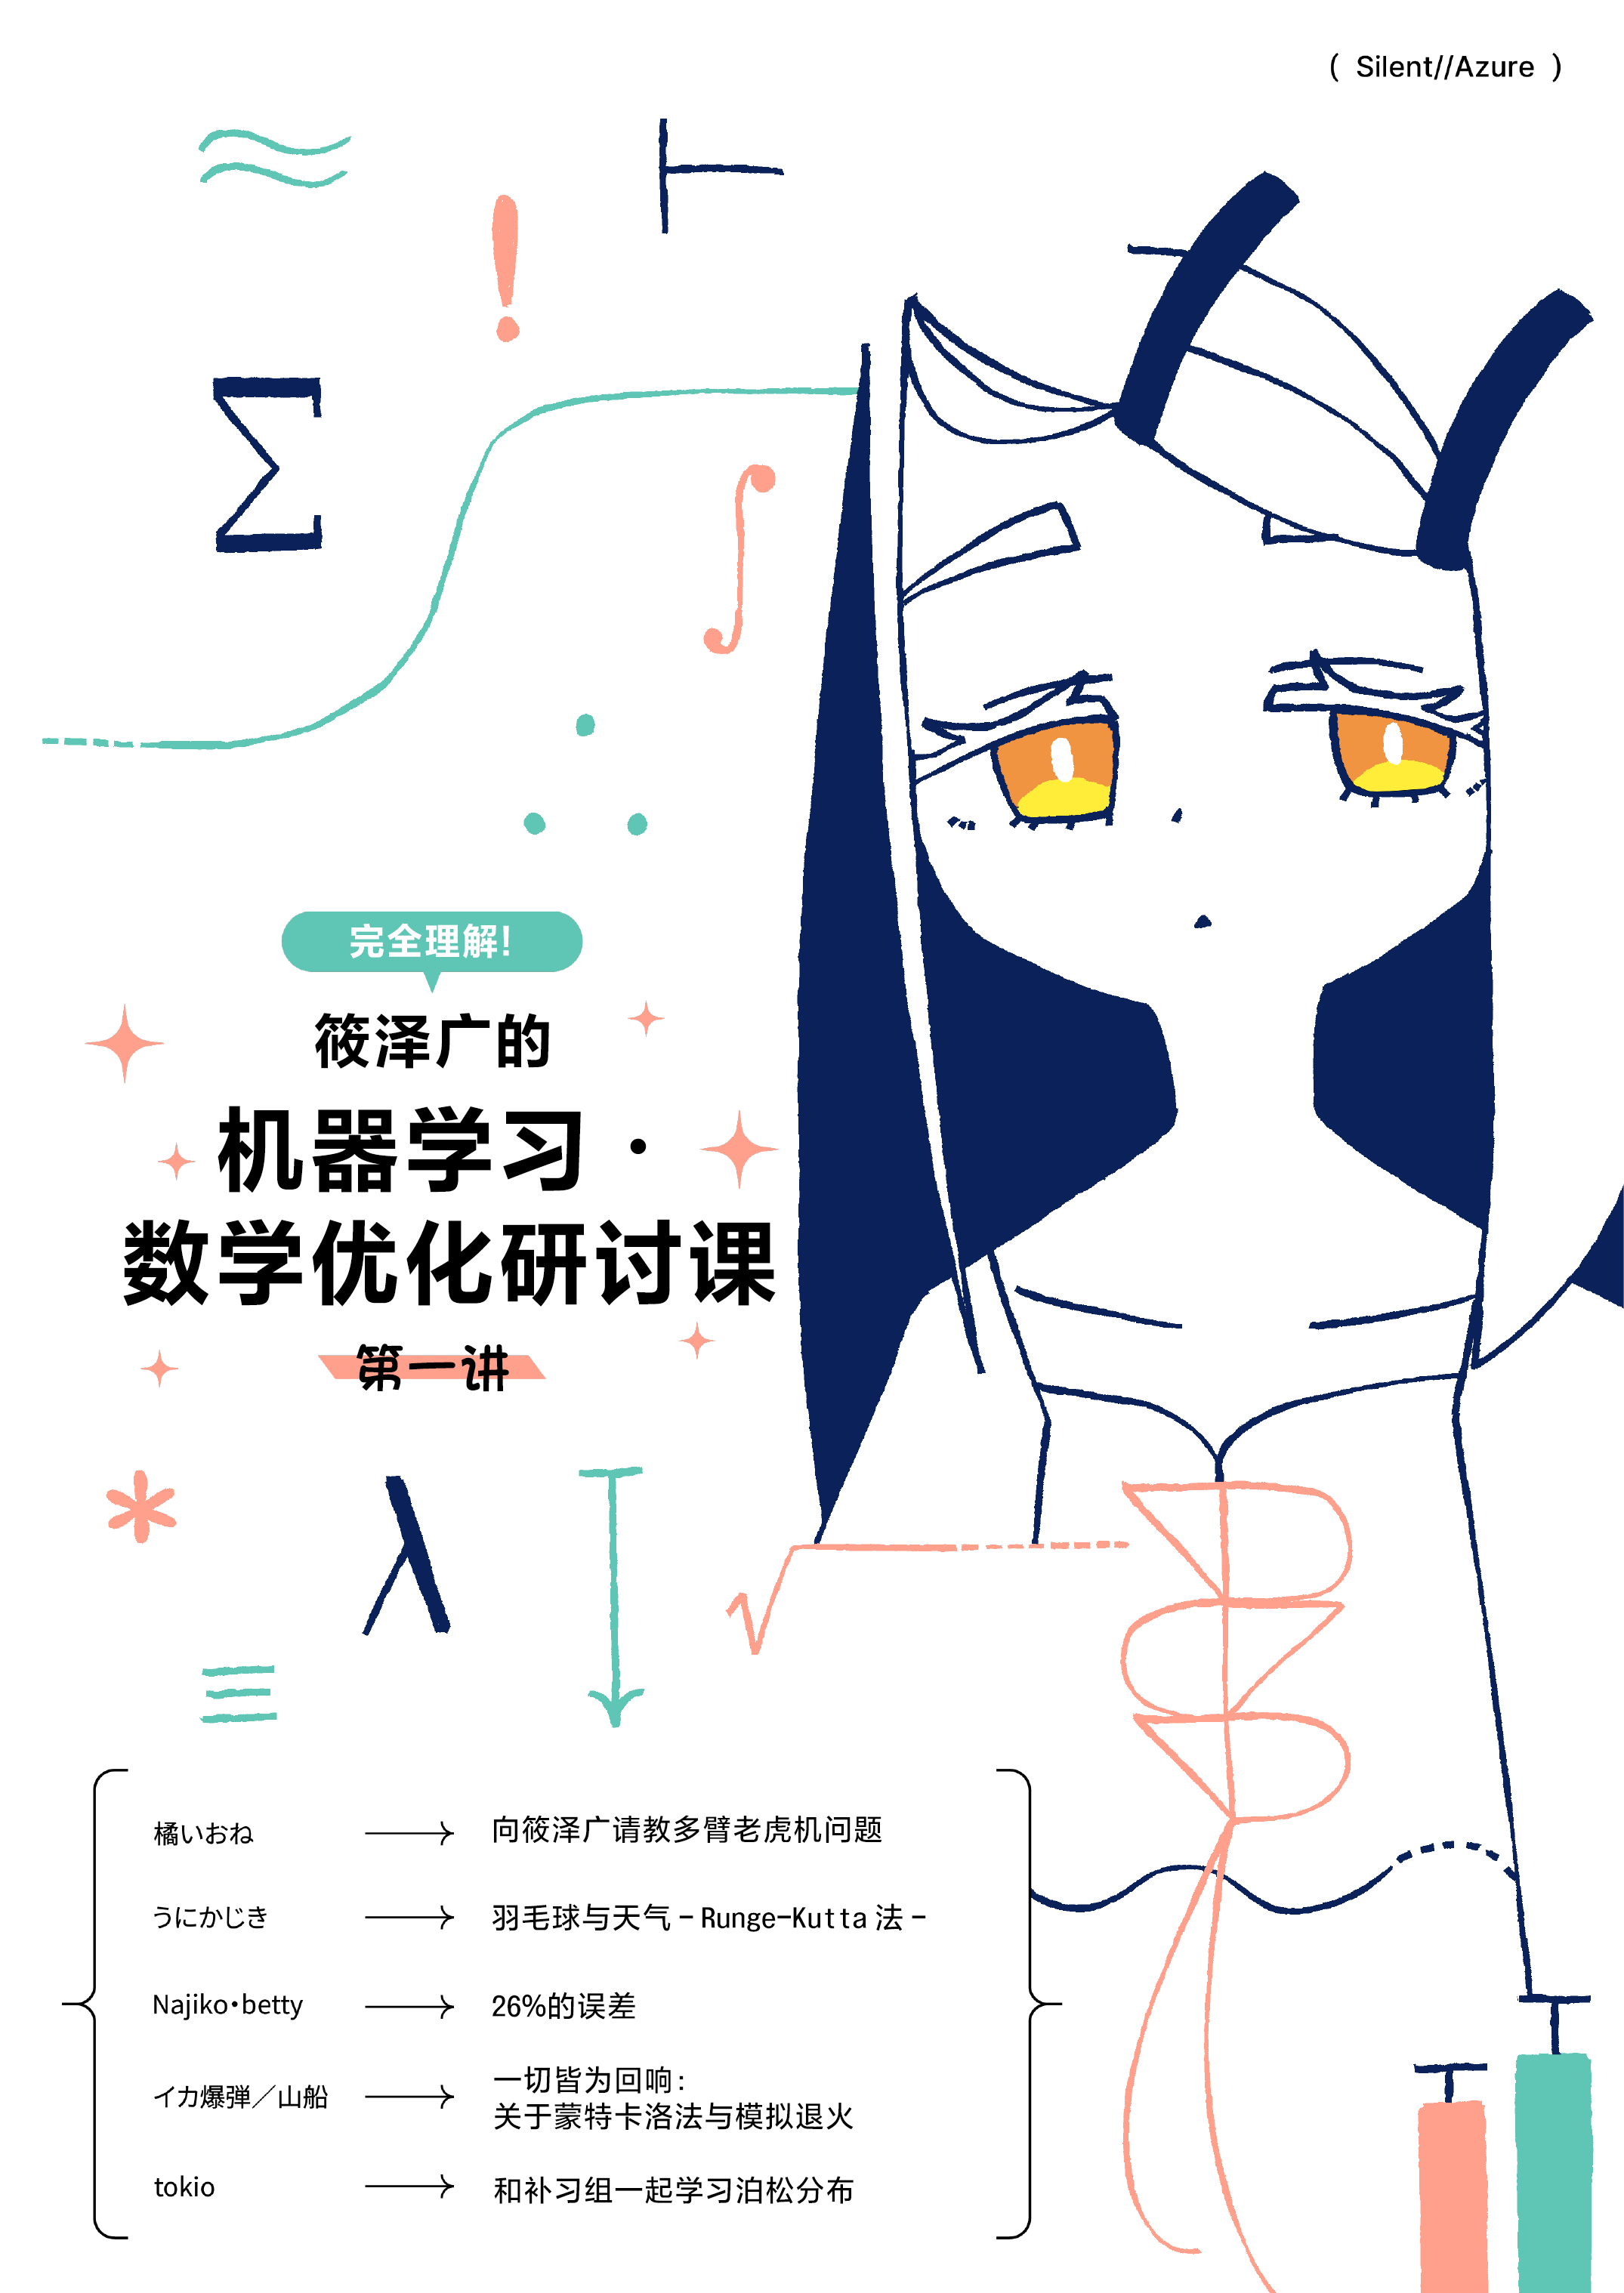
\includegraphics[width=0.92\textwidth]{figures/extracted/ml-optimization-seminar-1/cover.png}
\end{figure}
\clearpage
\section*{向筱泽广请教多臂老虎机问题}
\addcontentsline{toc}{section}{向筱泽广请教多臂老虎机问题}
\begingroup\small
\noindent\textit{来源：docs/完全理解！筱泽广的机器学习$\cdot$数学优化研讨课\textasciitilde{}第一讲\textasciitilde{}/1.向筱泽广请教多臂老虎机问题.pdf；页数：10；可抽取文字页：10。}\par
\endgroup
\medskip
\begingroup
\setlength{\parindent}{0pt}
\setlength{\parskip}{0.45em}

% --- PDF page 1 ---
向筱泽广请教多臂老虎机问题\par
序章\par
在五月的一个格外炎热的日子里，我皱着眉头盯着电脑屏幕。偶尔往表格软件里敲入几\par
个数字，又把它们全删掉，双臂抱胸靠在椅背上。就是这样一个烦人的下午。\par
坐在一旁一直盯着我的筱泽同学，终于开口了。\par
「今天的制作人看起来比平时还要愉快呢。怎么了？ 」\par
「其实，我在为 SNS 上的广告发愁。面对三种不同的广告，不知道该如何分配预算。 」\par
「嗯嗯。——制作人，我来给你上一堂课吧。 」\par
「上课？ 」\par
「嗯。关于如何用数学的方法来决定广告预算分配。 」\par
筱泽同学从桌下的包里拿出一本笔记本，站起身坐到我旁边。淡雅的香水味静静地宣告\par
着她的存在。\par
「首先我们要从问题的定义开始。现在，制作人手上有三种广告。目标是尽可能把预算\par
分配给效果最高的广告。但目前还不知道哪种广告最有效，对吧？ 」\par
筱泽同学微微歪了下头。\par
「没错。一般来说，广告效果是通过展示数与点击数来计算的。可这次是 SNS 广告，所\par
以还要包括点赞、新关注等在内，提高整体点击率才是主要目标。 」\par
「OK——那就开始上课，吧。 」\par
「在进入正题前，先整理一下专有名词吧。制作人正在烦恼的广告预算分配问题，其实\par
可以解释为\par
Multi-Arm Bandit\par
多臂老虎机问题。 」\par
「Multi-Arm Bandit 问题——听起来不像是关于有很多胳膊的\par
Bandit\par
盗贼的故事啊。 」\par
「呵呵，制作人真有趣呢。——这里所说的 Bandit 指的是老虎机。不过，这台老虎机\par
有\par
Multi-Arm\par
好几根拉杆，而且每一根拉杆中奖的概率都不一样。我们的目标，就是要在其中找出\par
中奖概率最高的拉杆。 」\par
「原来如此。广告的种类就是拉杆的数量，而用户的点击就相当于中奖。 」\par

% --- PDF page 2 ---
「正解。 那我来出一道题吧。 想找出三种广告里最有效的那一个时， 制作人会怎么做呢？ 」\par
「凭直觉的话， 『把所有广告都投一段时间，然后检测结果』 ，大概会这么做吧。 」\par
「的确，全都试一试是一种有效的策略。但像这次这样时间和预算都有限的情况下，就\par
行不通了。所以我们就要引入\par
Exploration\par
探索 和\par
Exploitation\par
利用的概念。 」\par
「在多臂老虎机问题中，探索就是去拉那些中奖概率还不清楚的拉杆。也可以说是为了\par
将来获得更大利益而进行的信息收集。而利用则是反复拉当前表现最好的拉杆。可以把\par
它视为为了短期利益最大化的行为。 」\par
「关键就在于探索与利用的平衡。用广告作例子吧。如果广告 A 投了几次效果不错，而\par
平衡偏向了利用一方，会发生什么呢？ 」\par
「利用追求的是短期利益……所以会放下广告 B 和 C，只是一味地继续投放广告 A 吧。 」\par
「没错。如果广告 A 确实是最有效的，那当然没问题。但要是广告 B 或 C 更有效的话，\par
结果就是吃亏。找到探索与利用的最佳平衡，这正是多臂老虎机问题的核心。 」\par
「多臂老虎机问题我已经理解了——那么探索与利用的平衡该如何计算呢？ 」\par
「好问题啊。 」筱泽同学露出有些高兴的表情。 「接下来就来看看实际的计算公式吧。 」\par
「首先，让我们试着用数学公式来描述多臂老虎机问题。可能有点难，但还请忍耐一下，\par
哦。 」\par
说着，筱泽同学在笔记本上写起了公式。笔尖在纸面上舞动，墨迹逐渐化作一行行数学\par
表达。\par
「我们能够选择的选项集合， 用集合K 来表示。比如有广告 A、B、C 时，K = A, B, C。\par
相对地，K 中的每个广告就是 k，如果要强调它属于 K，就写成 k$\in$ K。 」\par
「每一次试验用时间 t 来表示。广告的情况下， t = 1 就是第一次投放，t = 2 是第二次\par
投放……依此类推。 」\par
「在时刻 t 被选中的选项写作 at。比如 a1 = A，意思就是『第一次投放展示了广告 A』 。 」\par
「广告是否被点击用 rt 表示——即在第 t 次投放 at 时是否得到了『点赞』或新关注。如\par
果有回报就是 rt = 1，没有就是 rt = 0。 」\par
「每个广告的真实回报概率，也就是点击率，用 $\mu$k 表示。比如广告 A 的点击率是 10\%，\par
就写成 $\mu$A = 0.1。不过 $\mu$k 是『真实』概率，我们一开始并不知道。 」\par

% --- PDF page 3 ---
「我们的目标，是在总试验次数为 T 时，让总回报 $\sum$T\par
t=1 rt 最大化。这里的 $\sum$ 是『求\par
和』的符号，在数学里常用来表示连续值的累计。 」\par
「求和，也就是 $\sum$T\par
t=1 rt，等于 r1 + r2 +$\cdot$$\cdot$$\cdot$ + rT 。用中文写出来就是『把第 1 次到第 T\par
次的所有回报全部加在一起』 ，对吧。 」\par
「不愧是制作人，理解得真快，帮大忙了。问题的说明到此结束，接下来就进入解法吧。\par
首先从最基础的算法——\textbf{[缺字]}-greedy 法开始讲解。 」\par
「所谓 $\epsilon$-greedy 法，顾名思义，就是始终\par
greedy\par
贪心地选择当前成绩最好的选项。但如果仅仅\par
这样，可能会错过真正的最优解，所以就用概率 $\epsilon$ 随机尝试其他选项，从而进行适度的\par
探索。$\epsilon$ 是 0 到 1 之间的小数——比如 0.1。如果这个值大， 就偏重探索； 如果值小， 就\par
偏重利用。 」\par
「在时刻 t 选择选项 k 时得到的平均回报 $\mu$k 的估计值记作 ˆ$\mu$k(t)。上标 ˆ$\cdot$ 常用于表示估\par
计值，记住这个符号就好。ˆ$\mu$k(t) 的计算公式如下」\par
ˆ$\mu$k(t) =\par
$\sum$t-1\par
i=1 ri$\cdot$ I(ai = k)$\sum$t-1\par
i=1 I(ai = k)\par
「式中出现的这个叫做\par
Indicator function\par
指示函数， 当括号里的条件为\par
T rue\par
真时返回 1， 为\par
F alse\par
假时返回 0。制作人，\par
你知道 I(ai = k) 的意思吗？ 」\par
「意思是，在第 i 次试验中，如果选择了 k 就那它是 1，否则就是 0，对吧。 」\par
「没错。也就是说，公式中的分子 $\sum$t-1\par
i=1 ri$\cdot$ I(ai = k)，表示『在过去每次试验中，如果选\par
择了 k，就把当时得到的回报 ri 加起来』 ，最终得到的是『从选项k 获得的回报总和』 。 」\par
「分母 $\sum$ i = 1 t-1I(ai = k)，表示『在过去的每次试验中，如果选择了 k，就加 1』 ，最终\par
得到的是『选择 k 的总次数』 。那么ˆ$\mu$k(t) 公式计算出来的就是——」\par
筱泽同学停下话语，微笑着看向我。不知道她是想确认我的理解程度，还是单纯想让我\par
困惑。我心里这样想着，接过了剩下的话。\par
「——就是把至今从选项 k 得到的回报总和，除以选择 k 的总次数——换句话说，就是\par
『选项 k 的平均回报』 。 」\par
我也从笔筒里拿起一支圆珠笔，在筱泽同学写下的公式下添上新的式子。\par

% --- PDF page 4 ---
ˆ$\mu$k(t) = 到时刻t- 1为止从选项k得到的回报总和\par
到时刻t- 1为止选择k的总次数\par
「答对了。所以 ˆ$\mu$k(t) 就是『下次选择 k 时，根据以往经验，大概会得到这样的回报』的\par
预测。——对了制作人，要是选择 k 的次数是零，会怎样呢？ 」\par
「分母变成 0，就会出现除以零……那就没法计算了。 」\par
「正是如此。所以在计算 ˆ$\mu$k(t) 时要动些脑筋。比如在计算前，先让每个选项至少被选择\par
一次；或者，把还没选过的选项的 ˆ$\mu$k(t) 设置成一个非常大的值。 」\par
「在 $\epsilon$-greedy 法中，会用到这些公式和变量，并根据以下规则来选择行动:」\par
1. 生成一个 0 到 1 之间的随机数。\par
2. 如果随机数小于 $\epsilon$，就从所有选项 K 中随机选择一个。\par
3. 如果随机数大于等于 $\epsilon$，就选择 ˆ$\mu$k(t) 最大的选项。\par
「第 3 步用公式表示就是： at = arg maxk$\in$K ˆ$\mu$k(t) 其中 arg max 表示『从给定的范围中，\par
选出使后面公式值最大的那个参数』 。现在我们把这个行动原则套用到广告上来想一想\par
吧。 」\par
1. 有广告 A、B、C，且 $\epsilon$ = 0.1。\par
2. 而且到目前为止，广告 A 的点击率最高。\par
「这种情况下，广告投放会怎么决定呢？ 」\par
「因为 $\epsilon$ = 0.1，即有 10\% 的概率进行探索，所以会有 90\% 的概率投放广告 A，而剩下\par
10\% 的概率会在 A、B、C 中随机选择一个投放。 」\par
「嗯，理解得很到位呢。最后我来总结一下 $\epsilon$-greedy 法的优点与缺点吧。 」\par
$\epsilon$-greedy 法的优点：\par
• 思路直观，容易理解。\par
• 实现非常简单。\par
$\epsilon$-greedy 法的缺点：\par
• 在探索时完全随机，所以即使表现很差的选项也会以相同概率被选中。\par
• 很难选出最优的 $\epsilon$ 值。注 1\par
「那么问题来了，制作人。如果要想办法消除 $\epsilon$-greedy 法的缺点，你会怎么做呢？ 」\par
「我想……探索时与其完全随机选择，不如优先选择尝试次数少的选项。即便成绩看起\par
来一样，与其重复选择已经试过很多次的，不如去检验那些结果还不确定的，更加合理\par

% --- PDF page 5 ---
吧。 」\par
「很好的思路。接下来，就来讲把这种思路形式化的算法——UCB。 」\par
4\par
「UCB，也就是 Upper Confidence Bound 算法，是一种基于『乐观估计』来选择选\par
项的算法。它认为『试验次数少的选项，依然可能隐藏着较大的回报潜力』 ，因此在每\par
个选项的估计回报 ˆ$\mu$k(t) 上加上一个“不确定性奖励” ，以此作为评价标准。而这个奖\par
励，就是所谓的上限置信区间——Upper Confidence Bound 。 」\par
筱泽同学在“Upper Confidence Bound ”的字上标注了「上限置信区间」作为注解。\par
「置信区间，是统计学上的一个术语，表示『真实值有很高的概率——比如 95\%——会\par
落在这个区间中』 。比如一枚硬币只投了一次就正好是正面，若断言『这枚硬币正面概\par
率是 100\%』显然很危险。实际上，可能只是正反各半的硬币碰巧偏了一下。置信区间\par
就是用数值去表示这种不确定性的方法。试验次数少的选项不确定性大，区间就更宽；\par
试验次数多、可信度高的选项区间就更窄。而 UCB 算法，就是把这个区间的上限当作\par
乐观指标来使用。 」\par
「原来如此。引入 UCB 后，不仅成绩好的选项有机会被选，试验次数少、仍有未知潜力\par
的选项也能被关注。换句话说，就是能更好地平衡探索与利用。 」\par
「没错。在时刻 t 时，选项 k 的得分 U CBk(t) 的计算公式如下 注 2 。这里 ˆ$\mu$k(t) 的计算\par
方式与 $\epsilon$-greedy 时相同。 」\par
U CBk(t) = ˆ$\mu$k(t) +\par
$\sqrt{}$\par
c ln t\par
Nk(t- 1)\par
「来解释一下符号。首先，Nk(t- 1) 表示到时刻 t- 1 为止，选项 k 被选择的次数。 」\par
「ln t 是时刻 t 的自然对数。细节就省略了，这里只要知道随着 t 变大，ln t 的增长会变\par
缓，从而避免“不确定性奖励”无限膨胀，盖过了平均回报 ˆ$\mu$k(t)。 」\par
「c 是调整探索积极性的常数。按照最初提出该公式的论文，通常取 c = 2。 」\par
「根号$\sqrt{}$$\cdot$ 的作用，就是让不确定性奖励的增长率变得平缓。 」\par
「如果把这个“不确定性奖励”的公式翻译成自然语言，大概就是这样」\par
Bonus =\par
$\sqrt{}$\par
探索常数c$\times$ 试验次数t的自然对数\par
到时刻t- 1为止选择k的总次数\par

% --- PDF page 6 ---
「不过，这个公式在计算得分时有个问题。制作人，你能指出来吗？ 」\par
「嗯。我想这里和 ˆ$\mu$k(t) 一样，当选项 k 的试验次数为零时，分母 Nk(t- 1) 就变成 0，\par
无法计算 c ln t\par
Nk(t-1) 。 」\par
「对，没错。所以在 UCB 算法里，同样需要在最初先尝试所有选项一次，用来初始化得\par
分。 」\par
「用 UCB 算法来求解多臂老虎机问题时，它的行动原则与 $\epsilon$-greedy 大致相同。在\par
时刻 t，计算所有选项的 U CBk(t)，选出最大的那个作为 at。公式表示就是： at =\par
arg maxk$\in$K U CBk(t) 」\par
「那么，现在来试一道练习题吧。 」\par
1. 有广告 A、B、C，c = 2，t = 100。\par
2. 到时刻 t- 1， 广告A 累计展示 80 次 （NA(100) = 80 ） ， 平均点击率50\%（ˆ$\mu$A(100) =\par
0.5） 。\par
3. 到时刻 t- 1， 广告B 累计展示 10 次 （NB(100) = 10 ） ， 平均点击率10\%（ˆ$\mu$B(100) =\par
0.1） 。\par
「请计算此时广告 A 和 B 的得分 U CBA(100) 与 U CBB(100)。 目标是理解公式， 用计算\par
器也没问题，哦。 」\par
筱泽同学指了指笔记本的空白处。我打开电脑上的计算器应用，开始解题。\par
「因为 ln 100$\approx$ 4.605，代入公式 U CBk(t) = ˆ$\mu$k(t) +\par
$\sqrt{}$\par
c ln t\par
Nk(t-1) ……」\par
U CBA(100)$\approx$ ˆ$\mu$A(100) +\par
$\sqrt{}$\par
2$\times$ 4.605\par
80\par
= 0.5 +\par
$\sqrt{}$\par
2$\times$ 4.605\par
80\par
= 0.5 +\par
$\sqrt{}$\par
9.21\par
80\par
= 0.5 +\par
$\sqrt{}$\par
0.115125\par

% --- PDF page 7 ---
「\par
$\sqrt{}$\par
0.115125$\approx$ 0.339，所以 U CBA(100)$\approx$ 0.839。接下来是广告 B……」\par
U CBB(100)$\approx$ ˆ$\mu$B(100) +\par
$\sqrt{}$\par
2$\times$ 4.605\par
10\par
= 0.1 +\par
$\sqrt{}$\par
2$\times$ 4.605\par
10\par
= 0.1 +\par
$\sqrt{}$\par
9.21\par
10\par
= 0.1 +\par
$\sqrt{}$\par
0.921\par
「因为\par
$\sqrt{}$\par
0.921$\approx$ 0.96，所以 U CBB(100)$\approx$ 1.06。 」\par
「啪唧啪唧。做得很好。这里要注意的是，广告 B 虽然平均回报比广告 A 差，但在得\par
分上却超过了广告 A。这就是 UCB 算法的特征——不仅考虑平均回报，还考虑不确定\par
性。 」\par
「在进入下一个解法之前，先复习一下 UCB 算法的优缺点吧。 」\par
UCB 算法的优点：\par
• 与 $\epsilon$-greedy 中难以设定的 $\epsilon$ 不同，UCB 有推荐的探索常数取值。\par
• 实现非常简单。\par
UCB 算法的优点：\par
• 相比 $\epsilon$-greedy，计算更复杂一些。\par
• 在奖励不局限于 [0, 1] 的情况下（比如广告收益金额） ，效果不好。注 3\par
「顺便一提， 这种『因为没有选择最优选项而导致的损失』有个名字， 叫做\par
Regret\par
累计遗憾。在\par
部分优化问题中，目标不是最大化收益，而是最小化累计遗憾。 」\par
「那么，最后再讲一个方法——汤普森采样，用它来为这堂课收个尾吧。 」\par
5\par
「\par
Thompson Sampling\par
汤普森采样 注 4 是基于贝叶斯统计思想的算法。制作人，你懂贝叶斯统计吗？ 」\par
「只懂一点点……大概就是『用实际观测值不断更新下一次预测值』的循环，对吧。 」\par
「能理解到这一步就足够了。其实我很想从贝叶斯定理开始仔细解释，但今天就先省略\par
吧。 」\par
「——在汤普森采样中，会考虑『每个选项的真实回报概率 $\mu$k 大约会某种概率取到这个\par

% --- PDF page 8 ---
值』这样的分布。 」\par
「然后，每次选择一个选项并得到回报后，就用结果去更新分布。而在做选择时，则从\par
每个选项的分布中\par
采样\par
随机抽取一个样本，取样值最大的那个选项作为最终决策。 」\par
筱泽同学翻开笔记，在上面画出了几个山形的曲线，有的低而宽缓，有的高而尖锐。那\par
流畅的曲线让我忍不住去想象，她在与我相遇之前，就已经习惯画这种图景了吗。\par
「试验次数少、对真实回报概率信心不足的选项，它的分布范围很宽，从小值到大值都\par
可能被采样到。相反，试验次数多、信心度高的选项，分布的山会变得狭窄尖锐，更容\par
易采样到接近平均回报预测值 ˆ$\mu$k 的数值。 」\par
「分布范围宽的选项，其采样值有可能大幅高于 ˆ$\mu$k。所以，就像 UCB 一样，试验次数\par
少的选项也能压过已有成绩的选项，获得被选中的机会。 」\par
「没错。不过与 UCB 不同，汤普森采样并不是人为给探索次数少的选项加奖励，所以如\par
果成绩差，即使试验次数少，也会逐渐被忽略。而且不需要像 \textbf{[缺字]}-greedy 的 \textbf{[缺字]} 或 UCB 的\par
参数那样额外设值，它会自然收敛到最优解，这就是汤普森采样的特点。 」\par
「那么来看实际的公式吧。如果像广告这种，回报能分为 0 或 1 的情况，就叫『伯努利\par
老虎机』 。在这种情况下，通常会用Beta 分布来描述选项的真实回报概率 $\mu$k。Beta 分\par
布写作 Beta($\alpha$k, $\beta$k)，由两个参数 $\alpha$k 与 $\beta$k 确定。 」\par
• $\alpha$k：在选项中观测到回报为 1 的次数 + 1\par
• $\beta$k：在选项中观测到回报为 0 的次数 + 1\par
「给初始值加 1，是为了让最开始的分布比较平坦。因为在什么都没尝试之前，我们根本\par
不知道 $\mu$k 会取什么值。制作人，如果反过来想，会怎样？ 」\par
「就意味着——所有的值都是等可能的。 」\par
「答对了。 」筱泽同学微微眯起眼睛，露出一丝笑容。 「那我们来整理一下汤普森采样的\par
步骤吧。 」\par
1. 对于时刻 t 的每个选项，从它当前的 Beta 分布 Beta($\alpha$k, $\beta$k) 中随机采样样本值 $\theta$k。\par
2. 选择样本值最大的那个选项：at = arg maxk$\in$K $\theta$k。\par
3. 执行选中的 at，并观测报酬 rt。\par
4. 根据观测结果，更新 at 的 Beta 分布：\par
• 如果 rt = 1（获得报酬） ，则更新$\alpha$at← $\alpha$at + 1。\par
• 如果 rt = 0（未获得报酬） ，则更新$\beta$at← $\beta$at + 1。\par
「汤普森采样的讲解就到这里。——那么最后，来出一道稍微难一点的题吧。 」\par
筱泽同学带着一点恶作剧的笑容，在笔记本上写下了新题目。\par

% --- PDF page 9 ---
作业：用 Beta 分布进行广告效果的置信度分析\par
• 你已经连续投放了两周广告，目前各广告的 Beta 分布参数如下：\par
– 广告 A：$\alpha$A = 23, $\beta$A = 77\par
– 广告 B：$\alpha$B = 8, $\beta$B = 12\par
– 广告 C：$\alpha$C = 5, $\beta$C = 45\par
• 问 1：计算各广告的点击率期望（均值）与方差。已知 Beta 分布 Beta($\alpha$, $\beta$) 的均值\par
为 $\alpha$\par
$\alpha$+$\beta$ ，方差为 $\alpha$$\beta$\par
($\alpha$+$\beta$)2($\alpha$+$\beta$+1) 。\par
• 问 2：对于广告 A 与广告 B，求「真实点击率 $\mu$A > $\mu$ B 的概率 P ($\mu$A > $\mu$ B)」 。\par
• 问 3：综合考虑广告当前的表现、置信度以及未来的探索价值，作为制作人，你将如\par
何制定明天的广告投放策略？请给出理由。\par
「明天上课前解出来吧。制作人一定能做到的。 」\par
「呵呵……我很期待哦。 」\par
参考文献\par
Auer, Cesa-Bianchi, and Fischer: Finite-time Analysis of the Multiarmed Bandit Problem ,\par
2002\par
脚注\par
1.「像是这个问题的处理方法 $\epsilon$t = $\epsilon$0\par
t 这样随着试验次数增加而减少 $\epsilon$ 的 $\epsilon$ 调度（$\epsilon$-\par
scheduling）经常被使用。这样做可以在开局阶段大胆地进行探索，并在终局阶段更\par
偏向于利用来进行收敛。 」\par
2.「在“Finite-time Analysis of the Multiarmed Bandit Problem ”这篇论文中提出的\par
UCB 计算公式有 UCB1、UCB2、UCB1-NORMAL、UCB1-TUNED 这 4 种，不过\par
这次我们用 UCB1。 」\par
3.「这种情况下，通常会用 UCB-NORMAL 或 UCB-TUNED 来代替 UCB1。 」\par
4.「它也被称为概率匹配或后验采样。 」\par

% --- PDF page 10 ---
译者：\par
多臂老虎机是强化学习中最基础的模型哦。\par
另外关于广留下的作业这里给出思路：\par
1. 均值和方差怎么算都给了我还说啥了？带进去算就得了呗\par
2. 相信计算机吧，只管相信就是了（用蒙特卡洛模拟来跳过求解析解，最后的结果大约是\par
P ($\mu$A > $\mu$ B)$\approx$ 6.6\% ）\par
3. 由计算结果 B 的均值高但同时方差也大， A 的均值小方差也小， A 的收益可能大于 B ，\par
但 A 的收益大于 B 不太可能，C 更是路边一条，所以主攻 B ，次配 A ，看心情随便加\par
点 C\par
\endgroup
\clearpage
\section*{羽毛球与天气 - Runge-Kutta 法 -}
\addcontentsline{toc}{section}{羽毛球与天气 - Runge-Kutta 法 -}
\begingroup\small
\noindent\textit{来源：docs/完全理解！筱泽广的机器学习$\cdot$数学优化研讨课\textasciitilde{}第一讲\textasciitilde{}/2.羽毛球与天气 - Runge-Kutta 法 -.pdf；页数：27；可抽取文字页：27。}\par
\endgroup
\medskip
\begingroup
\setlength{\parindent}{0pt}
\setlength{\parskip}{0.45em}

% --- PDF page 1 ---
羽毛球与天气 - Runge-Kutta 法 -\par
うにかじき\par
「制作人。我要去体育馆」\par
在黑板前撑着讲台，白发少女这样说道。原本今天傍晚打算在房间里悠闲度过，却不知\par
不觉间要被自己的担当带偏了。\par
想象训练\par
平日的午后。正如前一天预报的一样，锋利的雨点从早晨起就不断地击打着地面，再加\par
上此时正值闷热的酷暑，穿行其中的走廊简直变成了地狱。\par
为了尽快逃离而快步走在笔直的走廊时，左眼瞥见了一间空荡荡的教室。在差点就要错\par
过的房间里，靠近窗边的座位上坐着一位少女，正是筱泽广。她双臂交叉放在桌上，像\par
是要一口吃掉一般正死死地盯着笔记本电脑的画面。那身姿，怎么看都不像十几岁的模\par
样。若是跳级十四岁就大学毕业，是否就能有她那般的氛围呢？\par
正思索着时， 才注意到她正在招手。 推开门， 踏入温度与湿度被空调调节到适宜的空间，\par
解放感自心中油然而生。\par
「你好，筱泽同学」\par
「你好，制作人」\par
关上门，互相交换了随意的问候，我走近筱泽同学。\par
「有什么事吗？ 」\par
「那是我才要问的。你一直在教室外盯着我看吧」\par
似乎是不自觉地盯着那副极具画意的坐姿看了太久。若是回答她的问题说「没什么事，\par
只是单纯在看」 ，总觉得有些难为情。正想着时，屏幕上排列的文字与图像映入眼帘。\par
「不，只是看你一直盯着电脑，不知道在想什么，所以产生了兴趣」\par
「这个吗？ 」\par
「是的。是某种程序吗？ 」\par
「嗯。我在计算羽毛球的轨迹」\par
「为什么要做这种东西？ 」\par

% --- PDF page 2 ---
「这周末要和千奈、佑芽出去玩，到时候会打羽毛球」\par
「你会打羽毛球吗？ 」\par
「至少应该不会成正式比赛吧。所以想多少练习一下。今天下雨，就用仿真来代替想象\par
训练了」\par
这是相当绕远的做法。普通人恐怕会看优秀选手的动作来做想象训练，而她却试图从物\par
理学里寻求指导。或许她早就察觉到了，网上随处可见的技巧和指导者，并没有考虑到\par
她那连站立都费力的体力不足。\par
「哪一条是羽毛球的轨道呢？ 」\par
「这条曲线就是从羽毛球左向右击出的轨道。 z = 0 m 上横向伸展的粗直线是羽毛球场，\par
差不多中间竖直伸出的直线是球网。这个图是从正侧面看球场的画面」\par
「曲线最后急剧弯曲的地方，真是像羽毛球一样的漂亮轨迹呢」\par
「因为加入了物理因素去仿真嘛。虽然比较粗略就是了」\par
「羽毛球会受到各种力的作用，但主要是朝向地面的重力和阻碍移动的空气阻力这两种。\par
把这些力写进运动方程，就变成右边的式子。解出来的，就是这个图」\par
她指着一本画有羽毛球图和公式的小笔记本。上面潦草写着的英文字母与符号，再夹杂\par
些许文字，透着浓浓的理科气息。\par
「真是复杂的公式呢。x, z 变成了什么式子？ 」\par

% --- PDF page 3 ---
「没有具体的解析式」\par
「诶？ 」\par
「要是想解，大概能解吧。但现在并没有推导出那种公式」\par
她轻易地说出了矛盾的话。\par
「没解出来的话，那刚才的仿真是怎么做的？轨迹都不知道啊」\par
「是强行让电脑去解的」\par
「啊啊，就是现在流行的 AI 吗」\par
「嗯...... 有点，不对，该说差得挺多吧。更准确地说，是把能用计算器算的方法，让电脑\par
自动而且高速地去做」\par
筱泽同学越是继续解释，仿真的原理就越让人不明白。明明没有解公式，却能做仿真？\par
明明是用电脑，为什么还要提计算器呢？\par
「\textbf{[缺字]}\textbf{[缺字]} 制作人。下午有安排吗？ 」\par
她似乎察觉到了我没有弄明白，望着教室的窗户这样问。\par
「没有，没别的安排」\par
「\textbf{[缺字]}\textbf{[缺字]} 不想试着理解一下这个仿真的内容吗？ 」\par
出现了——「陪我一小时」的宣言。眼前浮现出写满公式的整洁黑板。虽说有点提不起\par
劲，但接下来要做的也不过是整理资料，对仿真本身也并非毫无兴趣。更重要的是，从\par
自己担当那里得到授课的宝贵经历，可不是轻易能遇到的。比立刻回到地狱般的走廊要\par
好得多。\par
「也是呢。我很想理解一下」\par
「是吗。那么」\par
她从椅子上站起身，抱着电脑走向讲台，\par
「这是仿真中用到的数值计算方法之一」\par
捏起黑板上的剩余白粉笔，转身面对我，\par
「我要来讲解 Runge-Kutta 法的概要」\par
担当偶像的讲课，开始了。\par

% --- PDF page 4 ---
雨\par
「虽然有点突然，但我要把问题换成雨滴的下落哦」\par
「雨滴？ 」\par
「没错。 要表示羽毛球的轨道， 需要x, z 两个坐标轴。 相对地， 雨滴是从天空直直落到地\par
面，也就是只需一个轴就能仿真。比羽毛球少一个维度，所以更简单。而我现在要讲解\par
的 Runge-Kutta 法，两者都能用。用更单纯的雨滴作例子，能更容易理解仿真的内容」\par
「把问题换了，不会导致仿真出问题吗？ 」\par
「不能说完全没有这种可能。但雨滴的下落，和羽毛球的轨迹一样，主要作用力就是重\par
力和空气阻力。这是相似的情形，所以仿真也会类似，你就把它当成差不多就行了」\par
「原来如此。我明白了」\par
我点头同意后，她便走到黑板边缘，开始挥动粉笔。\par
「制作人，你知道雨滴大概以多快的速度落下来吗？ 」\par
「没想过呢……大概每秒几米左右？ 」\par
「直径 1 mm 的小雨大约就是这个速度。而直径 3 mm 的大雨，会以 8 m/s 的速度落下，\par
换算时速大概 30 km/h，就像住宅区里行驶的车速那样 [1] 」\par
「这么一听，比想象中要快啊」\par
「但另一方面，雨是从离地数千米的高空落下的 [2] 。这样想的话，只以车速落下，反而\par
显得慢了。你知道这是为什么吗？ 」\par
「因为在下落过程中，会受到空气阻力吧」\par
「答对了。 雨滴在下落过程中， 会因为空气阻力被刹住。 这种空气阻力和速度的平方成正\par
比，所以加速很快就结束了。实际上，掉落个 100 m 左右，雨滴的速度就几乎恒定了」\par

% --- PDF page 5 ---
m ˙v = -mkv 2 + mg\par
口头讲解告一段落后，她放下粉笔，转身看向我。\par
「刚才的内容，用写出动力学方程就是这样。我们把雨滴下落的方向定为 z 轴正向。雨\par
滴受到的力有两个：向下的重力、向上的空气阻力。把这两个写进动力学方程，就得到\par
了右边的式子。这里的符号代表速度对时间的微分，也就是加速度」\par
「就是 F = ma 那个吧」\par
「我们把等式两边都除以 m 化简。假设雨滴是自然落下，也就是初速度是 0 m/s 开始掉\par
下来的」\par
˙v = -kv 2 + g\par
翻页漫画\par
「解出这个式子，就能知道雨滴的下落速度。而现在的目的，就是要推导出让电脑计算\par
的方法。不过，这个式子没法直接丢给电脑算，所以得稍微改个形式」\par
「什么意思？ 」\par
「要方便电脑，把原本连续的数值拆成离散的。比如说……」\par
她从口袋里掏出手机，把镜头一下凑到我脸前，就这么静静拍了几秒。\par
「你在干嘛？ 」\par
「在拍制作人的视频。想着留作回忆」\par
「立刻删掉！ 」\par
「开玩笑的啦。接下来要用」\par
她这么一边说着，一边向我走来，把刚拍的视频递给我看。\par
「视频里的制作人，看起来是平滑地在动。但实际上，这视频只是每秒三十张照片快速\par
切换而已。原理和翻页漫画一模一样」\par
「这和你刚才的解释有什么关系？ 」\par
「你觉得在开始录像后的 1\par
60 秒时，制作人是不是也在动？ 」\par
「那当然是在动啊」\par

% --- PDF page 6 ---
「没错。 但这视频里， 并没有1\par
60 秒后的制作人。 因为这翻页漫画般的画面， 是每隔1\par
30 秒\par
才有一张，所以 1\par
60 秒的照片是不存在的」\par
话还没怎么接上，筱泽同学却已经从我身边离开。\par
「基本上，把现实中运动的物体交给电脑记录，数据也只能像翻页漫画那样被保存」\par
她重新转向黑板，开始画新的图。\par
「雨滴的下落速度，也得让电脑像翻页漫画一样去算。具体来说，就是每隔 h 秒只记录\par
一次速度。至于 h\par
2 秒后的速度，是不计算的」\par
「也就是说，只让它记下计算需要的地方，其他一律忽略，差不多是这种感觉吗？ 」\par
「差不多那样理解就行」\par
「可这样随意忽略，还能准确算出真实的速度吗？ 」\par
「嗯——应该说思路有点不一样吧。更接近的想法是，要想办法让电脑记下的速度，尽\par
量接近真实速度的数值」\par
啪嗒，传来一声干脆的轻响。\par
「为了后面的说明， 先给电脑要计算的速度值取个名字。 假设雨滴从开始下落， 每隔h 秒\par
的时刻是 0, h, 2h, 3h, ......, ih, (i + 1)h, ......。在这些时刻的速度分别是 v0, v1, v2, v3, ......,\par
vi, vi+1, ......。 其中v0 是初速度， 所以确定为0。 因此， 电脑需要计算的就是v1, v2, v3, ......,\par
vi, vi+1, ...... 这些」\par
定积分的近似式\par
「既然要让电脑算的数值已经定下了，接下来就要考虑具体的计算方法了」\par
「终于要进入正题了呢」\par
「没错。不过到现在为止，也才讲了两成左右而已」\par
看来她的宝贵授课还会继续下去。\par

% --- PDF page 7 ---
「先来看看最初的方程式。-kv 2 + g 是关于 t 的函数，所以我把它记作 f (t)」\par
˙v = -kv 2 + g = f (t)\par
「制作人，如果是你，要从这个式子里解出答案的话，会怎么做呢？ 」\par
「……完全没头绪」\par
「那就稍微岔开一点话题。如果是这个式子的话，你会怎么做？ 」\par
dy\par
dx = x\par
「两边对 x 积分就行吧」\par
「没错。具体写出来就是这样。C 是任意常数」\par
y =\par
Z\par
xdx = x2\par
2 + C\par
「运动方程式也能用类似的方式处理。由此就能导出 vi 和 vi+1 的关系」\par
＊　＊　＊\par
˙v 是 v 对 t 的微分。所以只要把右边的 f (t) 对 t 积分，就能得到 v。\par
v =\par
Z\par
f (t)dt\par
• 把 f (t) 的一个原函数记作 F (t)， 那么v 可以这样写。 因为f (t) 是关于 t 的函数， 所\par
以原函数用 t 来表示没有问题。\par
v = F (t) + C\par
当 t = ti, ti+1 时，就能分别得到 vi, vi+1。\par
8\par
<\par
:\par
vi = F (ti) + C\par
vi+1 = F (ti+1) + C\par
把这两个式子里的 C 消去，就能得到 vi+1 和 vi 的关系式。最后一步，用到了 F (t) 是\par

% --- PDF page 8 ---
f (t) 的原函数这一点。\par
vi+1 = F (ti+1) + vi - F (ti)\par
= vi + [F (t)]ti+1\par
ti\par
= vi +\par
Z ti+1\par
ti\par
f (t)dt\par
＊　＊　＊\par
「……右边的积分，要怎么计算呢？ 」\par
「这个定积分很难精确算出。所以，我们要想办法计算一个接近它的值，也就是近似值」\par
「……这就是之前说的， “想办法算出一个接近真实值”的意思吗」\par
「没错。在这一阶段，就彻底放弃去计算完美的下落速度」\par
这么说完后，筱泽同学再次向我抛出了问题。\par
「制作人，我再问一个问题。学数学时，用到定积分的时候，一般是在解什么题目？ 」\par
「只是普通的计算题……还有就是面积的计算吧」\par
「记得不错。没错，定积分可以用来算面积。这次的定积分值，其实就等同于这一部分\par
的面积」\par
「近似定积分，就是尽可能精确地去算这个面积。这里我介绍两种计算方法 [3] 」\par
＊　＊　＊\par
要求的面积，等于下文的 A 面积减去 B 面积。\par

% --- PDF page 9 ---
A 的面积 SA 用梯形的面积公式就能轻松算出。为了不让式子太繁琐，把 f (ti), f(ti+1)\par
简写成 fi, fi+1。\par
SA = h(fi + fi+1)\par
2\par
A 的面积看起来就很接近原定积分的面积。因此，可以用 SA 来近似定积分。这种近似\par
叫做台形法。这就是第一种计算方法。\par
Z ti+1\par
ti\par
f (t)dt $\simeq$ h(fi + fi+1)\par
2\par
如果能算出 B 的面积，就能更好地逼近定积分的面积。这里我们把 B 往下拉直。 （严格\par
说，是用 f (t) 去减去台形的斜边直线方程。 ）\par
拉直后的 B 所围成的曲线，可以用经过 (ti, 0), (ti, fc - fi+fi+1\par
2 ), (ti+1, 0) 三点的二次函数\par
来近似。因此就用这个二次函数来近似 B 的面积。曲线通过 (ti, 0), (ti+1, 0)，于是可以\par
用常数 $\alpha$ 写出二次函数：\par
y = $\alpha$(t - ti)(t - ti+1)\par
由于曲线过点 (tc, fc - fi+fi+1\par
2 )，可以确定 $\alpha$。\par

% --- PDF page 10 ---
fc - fi + fi+1\par
2 = $\alpha$(tc - ti)(tc - ti+1) = -$\alpha$ h2\par
4\par
$\Rightarrow$ $\alpha$ = - 4\par
h2\par
(\par
fc - fi + fi+1\par
2\par
)\par
= 2(fi - 2fc + fi+1)\par
h2\par
这样一来，二次函数就确定了。B 的面积 SB 可以近似为：\par
SB $\simeq$ -\par
Z ti+1\par
ti\par
$\alpha$(t - ti)(t - ti+1)dt\par
= $\alpha$ h3\par
6\par
= 2(fi - 2fc + fi+1)\par
h2\par
h3\par
6\par
= h(fi - 2fc + fi+1)\par
3\par
把 B 的面积从 A 的面积里减去，就能得到定积分的近似值。这种近似叫做辛普森公式。\par
这就是第二种计算方法。\par
Z ti+1\par
ti\par
f (t)dt = SA - SB\par
$\simeq$ h(fi + fi+1)\par
2 - h(fi - 2fc + fi+1)\par
3\par
= h(fi + 4fc + fi+1)\par
6\par
＊　＊　＊\par
「——以上就是台形法和辛普森公式两种近似公式。因为把 B 的面积扣掉了，辛普森公\par
式比台形法的精度更高」\par
近似精度的估算\par
「筱泽同学，可以问个问题吗？ 」\par
「怎么了？制作人」\par
「我大概能理解辛普森公式比台形法精度高，但到底能高多少呢？ 」\par

% --- PDF page 11 ---
「好问题。我正要讲这个呢」\par
「拜托了」\par
「要具体比较近似精度时，经常用到一个工具，叫做泰勒展开。所谓泰勒展开，就是把\par
f (t) 展开成 t 的多项式，像这样写。这里的 f (n)(ti) 指的是对 f (t) 关于 t 连续微分 n 次\par
后，再代入 ti 得到的值」\par
f (t) =\par
X\par
n=0\par
f (n)(ti)\par
n! (t - ti)n =\par
X\par
n=0\par
an(t - ti)n\par
(\par
$\forall$n $\in$ N, an = f (n)(ti)\par
n!\par
)\par
「所有函数都能这样展开吗？ 」\par
「当然有些函数不能。但现在你可以假设能展开。至于为什么能展开，理由太长，就省\par
略掉了」\par
「明白了」\par
「用这个公式，就能把刚才的定积分也近似算出来」\par
Z ti+1\par
ti\par
f (t)dt =\par
Z ti+1\par
ti\par
X\par
n=0\par
(an(t - ti)n) dt =\par
X\par
n=0\par
an\par
n + 1 hn+1\par
「这个式子，不是近似值，而是精确值，对吧？ 」\par
「没错。接下来我们算一下台形法和辛普森公式的结果。先把 fc, fi+1 展开一下」\par
fc =\par
X\par
n=0\par
an\par
2n hn, fi+1 =\par
X\par
n=0\par
anhn\par
「接下来计算台形法和辛普森公式」\par
h(fi + fi+1)\par
2 = f (ti)h + a1\par
2 h2 + a2\par
2 h3 + a3\par
2 h4 + a4\par
2 h5......\par
h(fi + 4fc + fi+1)\par
6 = f (ti)h + a1\par
2 h2 + a2\par
3 h3 + a3\par
4 h4 + 5a4\par
24 h5......\par
「把这两个近似式和精确值一比，就会发现台形法从 h3 项开始偏离，而辛普森公式是从\par
h5 项才开始偏离」\par
「……」\par

% --- PDF page 12 ---
「呵呵……制作人，你看起来很吃力啊」\par
比之前复杂得多的长公式，让我快要头晕目眩。我沉默着盯着黑板的样子，被她带着几\par
分羡慕的目光看着。\par
「虽然我没能跟上细节计算……但能明白两种近似的精度确实不同。光是多近似了 B 的\par
面积，就能让结果在 h3, h4 的项上保持一致，真厉害啊」\par
「嗯。而且还只是用了一条二次函数这种超级简单的曲线去近似而已」\par
「但是， 看起来好像辛普森公式反而更差啊……台形法是从h3 偏离， 辛普森公式是从h5\par
偏离，那不就意味着辛普森公式的偏差更大吗？ 」\par
「在仿真里，h 基本都会设定为小于 1。这样一来，就有 h5 < h 3，所以辛普森公式的误\par
差反而更小」\par
「所以 h 不能乱定？ 」\par
「没错。所以答案是——辛普森公式相比台形法有 h2 的精度提升。这就是对制作人问题\par
的回答」\par
fc, fi+1 的近似式\par
「我们再回顾一下辛普森公式吧」\par
Z ti+1\par
ti\par
f (t)dt $\simeq$ h(fi + 4fc + fi+1)\par
6\par
「你觉得右边这个式子，电脑能直接算出来吗？ 」\par
「应该不行。fc 是 f (c)，可电脑没法记住 tc 时刻的速度」\par
「没错。但我还是想办法让这个辛普森公式能用。要做到这一点，就得用 vi, fi 来近似\par
fc, fi+1」\par
「不只是 fc，连 fi+1 也要吗？ 」\par
「嗯。把 fi+1 也近似一下，就能得到电脑能处理的形式」\par
「这样一来，仿真就能跑了」\par
「没错。近似的时候，就用之前写下的 fc, fi+1 的泰勒展开」\par

% --- PDF page 13 ---
fc =\par
X\par
n=0\par
an\par
2n hn, fi+1 =\par
X\par
n=0\par
anhn\par
「这里把 fc, fi+1 展开到 h3 项为止，写成这样」\par
fc $\simeq$ fi + a1\par
2 h + a2\par
4 h2 + a3\par
8 h3\par
fi+1 $\simeq$ fi + a1h + a2h2 + a3h3\par
「你这删得可真狠啊，这样真的没问题吗？ 」\par
「没问题。把这个近似式直接代进辛普森公式，会变成这样。而且它和定积分的精确值\par
在 h4 项之前完全一致」\par
h(fi + 4fc + fi+1)\par
6 $\simeq$ fih + a1\par
2 h2 + a2\par
3 h3 + a3\par
4 h4\par
「本来辛普森公式也只在 h4 项之前能对得上，所以这样近似并没有破坏它的精度。因此\par
fc, fi+1 用到 h3 就足够了」\par
「原来如此」\par
「接下来，只要能把 f (1)(ti), f (2)(ti), f (3)(ti) 全都用 vi, fi 表示就行。这里直接利用 an 的\par
定义来算。先来求 f (n)，途中会用到 ˙v = f (t)。另外， ˙f 就是 f (1)(t)」\par
f (1)(t) = d\par
dt (-kv 2 + g) = d\par
dv (-kv 2 + g) $\cdot$ dv\par
dt\par
= -2kvf\par
f (2)(t) = d2\par
dt2 (-kv 2 + g) = d\par
dt (-2kvf )\par
= -2k( ˙vf + v ˙f )\par
= -2k(f 2 - 2kv 2f )\par
f (3)(t) = d3\par
dt3 (-kv 2 + g) = d\par
dt\par
(\par
-2k(f 2 - 2kv f )\par
)\par
= -2k\par
(\par
2f ˙f - 2k(2v ˙vf + v2 ˙f )\par
)\par
= -8k2(-2vf 2 + kv 3f )\par
「用这个就能得到 a1, a2, a3 如下」\par

% --- PDF page 14 ---
8\par
>>><\par
>>>:\par
a1 = f (1)(ti)\par
1! = -2kvifi\par
a2 = f (2)(ti)\par
2! = -k(f 2\par
i - 2kv 2\par
i fi)\par
a3 = f (3)(ti)\par
3! = - 4\par
3 k2(-2vif 2\par
i + kv 3\par
i fi)\par
「这样 a1, a2, a3 就能很漂亮地全都只用 vi, fi 算出来」\par
「没错。用这个近似式，fc, fi+1 就能与 vi, fi 有关。这样一来，定积分就能只用 vi, fi 这\par
两个量，通过辛普森公式求出来」\par
仿真的主要过程\par
「筱泽同学，前面一直在讲近似，但我还没看出这和仿真到底怎么联系起来……」\par
「抱歉。我来把流程整理一下吧」\par
不知不觉间，黑板七成都被泰勒展开和近似式填满了。最开始画的雨滴图，现在只剩下\par
角落里一点点，面积还不到公式的一半。\par
「首先，我们有动力学方程」\par
˙v = -kv 2 + g = f (t)\par
「把它改写成含定积分的形式」\par
vi+1 = vi +\par
Z ti+1\par
t1\par
f (t)dt\par
「首先用辛普森公式来近似右边的定积分」\par
vi+1 $\simeq$ vi + h(fi + 4fc + fi+1)\par
6\par
「接着，把 fc, fi+1 进一步用 vi, fi 来近似」\par

% --- PDF page 15 ---
8\par
>>><\par
>>>:\par
a1 = f (1)(ti)\par
1! = -2kvifi\par
a2 = f (2)(ti)\par
2! = -k(f 2\par
i - 2kv 2\par
i fi)\par
a3 = f (3)(ti)\par
3! = - 4\par
3 k2(-2vif 2\par
i + kv 3\par
i fi)\par
$\Rightarrow$\par
8\par
<\par
:\par
fc $\simeq$ fi + a1\par
2 h + a2\par
4 h2 + a3\par
8 h3\par
fi+1 $\simeq$ fi + a1h + a2h2 + a3h3\par
「通过对 fc, fi+1 的近似，辛普森公式就能完全用 vi, fi 来表示。这就是之前讲的全部内\par
容」\par
不必要的公式被大幅擦去，黑板一下空出了六成的空间。\par
「其实想做的事本身还挺简单的啊」\par
「只是计算过程繁琐而已，归根结底就是为了能让仿真跑起来而进行的近似」\par
「那么，怎么把这些真正落实到仿真里呢？ 」\par
「嗯，其实到这一步，用这个公式就能仿真雨滴的下落速度了」\par
「为什么呢？ 」\par
「首先要说明的是，fi 可以直接用 vi 算出来。 因为fi = f (ti) = -kv 2\par
i + g。 也就是说， 辛\par
普森公式只需要 vi 就能计算。有了这一点，vi+1 的近似值也就能只用 vi 来近似」\par
vi+1 $\simeq$ vi + h(fi + 4fc + fi+1)\par
6 = (仅和vi相关的式子)\par
「当 i = 0 时，v1 $\simeq$ (仅和v0相关的式子)。因为 v0 是初速度，给定为 0 m/s，所以能算出\par
v1。接着当 i = 1 时，v2 $\simeq$ (仅和v1相关的式子)，就能用刚算出的 v1 来得到 v2」\par
「也就是说，只要依次代入 i = 2, 3, 4, ......，就能像拔萝卜一样顺次得到 v3, v4, v5, ...... 的\par
值」\par
「没错。制作人，你领悟得挺快。这样一来， v1, v2, v3, ...... 全部都能算出来。顺带一提，\par
这正是为什么要近似 fi+1。因为普通的辛普森公式里，fc 和 fi+1 不能仅由 vi 得到，所\par
以才需要把它们都近似掉」\par
Runge-Kutta 法\par
「筱泽同学的仿真，就是根据这个公式跑的吗？ 」\par

% --- PDF page 16 ---
「不，我的不是用这个做的」\par
「不是这样吗？ 」\par
「嗯。因为这种方法有点不方便。要算 a1, a2, a3 的值，就得对 f (t) 求一阶、二阶、三阶\par
导数」\par
「确实，有点麻烦呢」\par
「而且如果 f (t) 换了，每次都得重新微分，那就太折腾了」\par
「也就是说，筱泽同学是用不求导的方法来近似的？ 」\par
「差不多是这个意思。具体来说，是从另一个角度来近似 vc, vi+1，最后让辛普森公式里\par
的 4fc + fi+1 在 h3 项为止一次对齐 [4] 」\par
「另一个角度？ 」\par
「刚才的方法，是用泰勒展开的式子去直接近似 fc, fi+1。接下来要讲的方式，不是靠公\par
式，而更像是从图形里去找相近的值」\par
「请看这个图。在时刻 tc 的速度记作 vc。这种方法的重点在于“斜率的接近” 。从ti 到\par
tc，再到 ti+1，它们的斜率（平均变化率）是这样的」\par
vc - vi\par
h\par
2\par
, vi+1 - vi\par
h\par
「这两个斜率，从图上看，都挺接近 ti 时的导数 ˙vi。接下来就是要利用这个……」\par
话还没说完，筱泽同学伸了个懒腰，看了看教室的时钟。犹豫了几秒后，她脚跟落下，\par
开始摆弄带到讲台上的电脑。\par
「这是？ 」\par

% --- PDF page 17 ---
「我在启动一个软件。接下来要计算 fc, fi+1 的近似精度，但公式变形太麻烦了。所以就\par
让一个叫 Maxima 的免费软件帮我全算掉」\par
「还有这么方便的软件啊」\par
「嗯……好了，准备完毕。那就回到正题吧」\par
她捏起一截短粉笔，转身面向黑板。\par
「先从 fc 的近似开始。根据刚才的思路，把 vc 的近似值记作 V1，算出来是」\par
V1 = vi + ˙vi $\cdot$ h\par
2 = vi + fi $\cdot$ h\par
2\par
「因为 ˙v = f (t) = -kv 2+g， 所以-kV 2\par
1 +g 应该就是 fc 的近似值。 把它记作F1 = -kV 2\par
1 +g，\par
并用 X1 表示它和 fc 的差」\par
fc = F1 + X1 = -kV 2\par
1 + g + X1\par
「把 X1 交给软件算……结果是这样。可以看出 F1 和 fc 在 h 项之前是吻合的」\par
X1 = - h2k2v2\par
i (kv 2\par
i - g)\par
2 + h3k2vi(kv 2\par
i - g)(3kv 2\par
i - 2g)\par
6\par
- h4k2(kv 2\par
i - g)(15k2v4\par
i - 15gkv 2\par
i + 2g2)\par
48 + ......\par
「马上就能算出来真方便啊」\par
「是啊，轻松多了」\par
「接下来要怎么做？ 」\par
「因为 F1 只对到 h 项，所以还要用“接近的斜率”再近似一下 fc。V1 接近 vc，另一方\par
面 ˙v = f (t) = -kv 2 + g，所以 F1 接近时刻 tc 的导数 ˙vc。如果 h 足够小， ˙vi 和 ˙vc 应该\par
差不多。因此 F1 也应当接近 ˙vi」\par
V1 $\simeq$ vc\par
˙vc = f (tc) = -kv 2\par
c + g\par
˙vi $\simeq$ ˙vc\par
9\par
>=\par
>;\par
$\Rightarrow$ ˙vi $\simeq$ -kV 2\par
1 + g = F1\par
「总之，就是把之前算出来的 fc 近似值 F1 当作斜率来用」\par

% --- PDF page 18 ---
「也就是说，把 V1 里用到的 ˙v1 换成 F1 吗」\par
「没错。于是 vc 的第二个近似值 V2 定义如下」\par
V2 = vi + F1 $\cdot$ h\par
2\par
「类似地，定义 F2, X2」\par
F2 = -kV 2\par
2 + g + X2\par
fc = F2 + X2\par
「把 X2 算出来的话……」\par
X2 = h2k2v2\par
i (kv 2\par
i - g)\par
2 - h3k2vi(kv 2\par
i - g)(3kv 2\par
i - 5g)\par
12\par
+ h4k2(kv 2\par
i - g)(3k2v4\par
i - 9gkv 2\par
i + 4g2)\par
48 + ......\par
「F2 也只对到 h 项啊。精度和 F1 一样吗？ 」\par
「不过如果把 X1, X2 结合起来，就能让 fc 对齐到 h2。先算 X1 + X2，其中 h2 的项会消\par
掉」\par
X1 + X2 = h3k2vi(kv 2\par
i - g)(3kv 2\par
i + 5g)\par
12\par
- h4k2(kv 2\par
i - g)(6k2v4\par
i - 3gkv 2\par
i - g2)\par
24 + ......\par
「因为 X1 = fc - F1, X2 = fc - F2，所以把它们代进去。把 X1 + X2 中 h3, h4 的系数分\par
别记作 P, Q」\par
fc - F1 + fc - F2 = P h3 + Qh4 + ......\par
$\Rightarrow$ fc = F1 + F2\par
2 + P\par
2 h3 + Q\par
2 h4 + ......\par

% --- PDF page 19 ---
「仔细一看，这个式子里 F1+F2\par
2 就已经能让 fc 对齐到 h2 项了」\par
「把之前的近似巧妙组合，就能提高 fc 的精度了」\par
「没错」\par
「那么接下来，就是用 F2 来近似 vc 再算 F3，然后把 F1, F2, F3 组合起来，让 fc 对齐到\par
h3 项，对吧？ 」\par
「我也想这么做，但很遗憾地告诉制作人，就算算出 F3，fc 的精度也不会再提高。这种\par
方法下，fc 的近似精度顶多只能到 h2」\par
「这样吗……」\par
「不过，还有 fi+1 的近似没做。这里定义 V3, F3, X3」\par
V3 = vi + F2 $\cdot$ h\par
F3 = -kV 2\par
3 + g\par
fi+1 = F3 + X3\par
「来算一下 X3」\par
X3 = - h3k2vi(kv 2\par
i - g)(3kv 2\par
i + g)\par
6\par
- gh4k2(kv 2\par
i - g)(3kv 2\par
i + g)\par
6 + ......\par
「F3 能对到 h2，但 h3 项还没消掉呢」\par
「不过，这个 h3 项其实能巧妙地消掉。制作人，你能想到吗？ 」\par
「不太能想出来……不过照刚才的思路，好像要和 X1, X2 组合起来？ 」\par
「不错，方向对了」\par
陌生的公式让我眼花缭乱。我从黑板下方往上，从右往左缓缓扫视，目光停在了其中一\par
个式子上。\par
「……原来如此。X3 的 h3 项，正好是 X1 + X2 的 h3 项的 -2 倍」\par
「不愧是制作人。 用这个就能把h3 消掉。 把2(X1 + X2) + X3 里 h4 的系数记作 R， 就有」\par

% --- PDF page 20 ---
2(X1 + X2) + X3 = Rh4 + ......\par
「像算 fc 的近似时那样来做吧。代入 X1 = fc - F1, X2 = fc - F2, X3 = fi+1 - F3」\par
2(fc - F1 + fc - F2) + fi+1 - F3 = Rh4 + ......\par
$\Rightarrow$ 4fc + fi+1 = 2F1 + 2F2 + F3 + Rh4 + ......\par
「左边这个式子是不是有点眼熟？ 」\par
「是筱泽同学之前说的，辛普森公式里没法直接算的那部分吧」\par
「对。那就代进去吧」\par
h(fi + 4fc + fi+1)\par
6 = h(fi + 2F1 + 2F2 + F3)\par
6 + Rh5\par
6\par
「这个式子说明， h(fi+2F1+2F2+F3)\par
6 和辛普森公式在 h4 项之前完全一致。之前说过，辛普\par
森公式就是把定积分逼近到 h4 的精度。所以用它替换辛普森公式，也能达到同样的精\par
度。把式子总结一下」\par
fi = -kv 2\par
i + g\par
$\Rightarrow$\par
8\par
>>><\par
>>>:\par
V1 = vi + fi $\cdot$ h\par
2\par
F1 = -kV 2\par
1 + g\par
V2 = vi + F1 $\cdot$ h\par
2\par
,\par
8\par
>>><\par
>>>:\par
F2 = -kV 2\par
2 + g\par
V3 = vi + F2 $\cdot$ h\par
F3 = -kV 2\par
3 + g\par
$\Rightarrow$vi+1 $\simeq$ vi + h(fi + 2F1 + 2F2 + F3)\par
6\par
「只要知道 vi， 就能顺序算出fi 到 F3， 再代进最后的公式， 就能得到vi+1 的近似值。 所\par
以从 v0 开始，就能逐次算出雨滴的下落速度。这种计算方法就叫做 Runge-Kutta 法」\par
「这个公式不需要对 f (t) 求导，只要直接用 f (t) 就行，确实轻松多了。这就是筱泽同学\par
用的方法吗？ 」\par
「没错。不过我的仿真是 x, z 双轴的。刚才推的是单轴的，所以稍微简单点。但也就是\par
式子多一些，原理和样子几乎一样」\par

% --- PDF page 21 ---
预测\par
「辛苦了。我的讲课到这里结束」\par
粉笔只剩一个指节长，她把它放下，拍了拍手，白色粉尘随之飞舞。\par
「筱泽同学也辛苦了」\par
「抱歉，没能讲到羽毛球的仿真。时间有点不够」\par
「不会的。光是雨滴就已经相当难了， 如果换成双轴， 我大概跟不上。不过， 筱泽同学用\par
的仿真理念和手法的大框架，我多少明白了」\par
「谢谢。你能这么说，我就觉得讲课有价值了」\par
「那用 Runge-Kutta 法算出来，雨滴的下落速度会怎样呢？ 」\par
「写到这一步做程序也用不了多久， 不如来试试看。 雨滴直径3 mm 时，k 大约是 0.15/m\par
[5] 。取 g = 9.8 m/s……」\par
她边说边用小手敲打键盘，过了一会儿就把屏幕转向我。\par
「嗯，搞定了」\par
「这是下落开始后几秒的速度变化。最初速度迅速上升，但到第 3 秒时差不多稳定在 8\par
m/s 了，不再增加。如果换算成下落距离，不到 50 m 加速过程就结束了」\par
「结果居然这么快就出来了啊」\par
「因为 Runge-Kutta 法本身算法简单， 程序也不会复杂， 所以很快就能出结果。 看吧， 还\par
不到五十行」\par
筱泽同学把程序给我看。\par
「真短啊，这样的话，感觉能很方便地算各种现象」\par

% --- PDF page 22 ---
「是的，只要公式明确就行。不过还需要正确的参数值」\par
「什么意思？ 」\par
「比如现在用的 k 值，就是直径 3 mm 雨滴专用的。直径变成 5 mm，就不能用了。而\par
且雨滴太大会变形，公式也得换 [6] 」\par
「那么，现在用的这些参数值，是怎么得到的呢？ 」\par
「是通过实验测出来的。实验观察到的下落速度，最符合的 k 值大约是 0.26 [7]」\par
「……那筱泽同学做的羽毛球仿真呢」\par
「当然是根据各种羽毛球的飞行实验得到的近似值。现在程序里是用那个 k 来设定的」\par
「原来如此。因为是对照了实验，所以仿真出的轨迹才那么像真的」\par
「没错。不过……」\par
她停顿片刻，拿起黑板擦，从上到下、从左到右把字迹抹去，接着继续说道。\par
「这个轨迹，只是羽毛球离开球拍之后的。至于发射角度和速度，是手动输入的参数」\par
「……那些参数是怎么定的？ 」\par
「角度会随持拍方式不同而变，没有固定值。速度取决于挥拍的快慢，也因人而异。某\par
些人甚至会出现完全不可能的参数组合吧」\par
「……那么，在羽毛球仿真里，你设的初速度是多少？ 」\par
「40 m/s。换算成时速就是 144 km/h」\par
「你觉得能打出这种轨迹吗？ 」\par
「基本不可能吧。手臂可能会碎掉呢」\par
「那，正确的数值是多少？ 」\par
「制作人啊。像样的参数基本都是实验得来的。但我羽毛球经验不多，所以哪些组合是\par
现实可行的，我也不清楚。所以——」\par
她擦完黑板， 从右侧回到中央， 在讲台前撑起双手， 这大概是她今天声音最坚定的一次：\par
「制作人。我们现在去体育馆」\par
「……哈？ 」\par
「去体育馆。借球拍，一边打羽毛球，一边找出参数的组合」\par
「我有必要跟去吗？ 」\par

% --- PDF page 23 ---
「我要你把我的羽毛球动作拍成视频，再配合仿真推算角度和初速度。拍视频得两个人，\par
所以你负责摄像」\par
「……我还有别的安排啊」\par
「记得一个小时前，你亲口说过下午没安排吧」\par
我真想揍一个小时前的自己。\par
「外面在下雨。我觉得天气好的时候练习，会更舒服吧」\par
我死马当活马医地反驳了一句，但她却露出胜券在握的笑容。\par
「也是呢。晴天会更好。那么……」\par
我们同时望向窗外，阳光正好从云缝里洒了进来。\par
「现在正合适呢」\par
看来老天是站在筱泽同学那边的。也可能是在对我说——认命吧。\par
「呐，制作人」\par
在我僵住时，眼前的女神温柔地说道：\par
「让电脑算出来的数值，几乎都会和真实值有偏差。参数一多，方程复杂起来，偏差就\par
会更大。厉害的人们一直在研究怎么把偏差尽量减小。我想天气预报就是个代表例子」\par
她接着说：\par
「即使预测精度不是 100\%，只要足够高，人们就能根据预测调整行动。今天讲的内容也\par
是一样，可以像看天气预报那样，随时决定要讲哪些，要省略哪些」\par
难道说——\par
「现在的天气预报，好像已经能预测到每小时的天气了。很厉害吧。据说预测精度大概\par
有 80\%，已经相当高了」\par
原来，我一直都在筱泽同学的手掌心里，被她耍得团团转。\par

% --- PDF page 24 ---
附录：落下速度的公式\par
「话说回来，雨滴的下落速度能作为公式直接解出来吗？ 」\par
「能的。我们来试试看吧」\par
＊　＊　＊\par
把 dv\par
dt 当作分数来处理，公式可以这样变形：\par
1\par
-kv 2 + g dv = dt\par
同时对两边做不定积分。左边可以化为如下形式。CL 为任意常数。\par
Z 1\par
-kv 2 + g dv =\par
Z 1\par
($\sqrt{}$g -\par
$\sqrt{}$\par
kv)($\sqrt{}$g +\par
$\sqrt{}$\par
kv)\par
dv\par
= 1\par
2$\sqrt{}$g\par
Z 1\par
$\sqrt{}$g -\par
$\sqrt{}$\par
kv\par
+ 1\par
$\sqrt{}$g +\par
$\sqrt{}$\par
kv\par
dv\par
= 1\par
2$\sqrt{}$gk ln\par
$\sqrt{}$g + v\par
$\sqrt{}$\par
k\par
$\sqrt{}$g - v\par
$\sqrt{}$\par
k\par
+ CL\par
右边为\par
R\par
dt = t + CR （CR 为积分常数） ，于是v 可得：\par
1\par
2$\sqrt{}$gk ln\par
$\sqrt{}$g + v\par
$\sqrt{}$\par
k\par
$\sqrt{}$g - v\par
$\sqrt{}$\par
k\par
+ CL = t + CR\par
$\Rightarrow$\par
$\sqrt{}$g + v\par
$\sqrt{}$\par
k\par
$\sqrt{}$g - v\par
$\sqrt{}$\par
k\par
= Ae2t$\sqrt{}$gk(A = e2(CR-CL)$\sqrt{}$gk)\par
$\Rightarrow$v =\par
r g\par
k\par
Ae2t$\sqrt{}$gk - 1\par
Ae2t$\sqrt{}$gk + 1\par
!\par
若为自然落下，即 t = 0 时 v = 0，则 A = 1。于是 v 的具体形式为：\par
v =\par
r g\par
k\par
e2t$\sqrt{}$gk - 1\par
e2t$\sqrt{}$gk + 1\par
!\par
＊　＊　＊\par

% --- PDF page 25 ---
「——就是这样」\par
「唔……老实说我没怎么听懂，不过至少公式能解出来就是了」\par
「对啊。比起羽毛球的要简单得多」\par
「既然 v 的公式能解出来，那用电脑算还有意义吗？ 」\par
「确实，像这次的雨滴例子就没什么麻烦」\par
她把手托在下巴上，嗯了一声，陷入思考。这副模样无论看多少次都格外迷人。\par
「来换个情况吧。真实的雨滴空气阻力已知既有速度的一次项，也有二次项。所以在运\par
动方程里加上 -mlv」\par
m ˙v = -mkv 2 - mlv + mg\par
「把这个 v 的方程硬解下去，结果会变成这样」\par
v = p+p-\par
( 1 - ek(p--p+)t\par
p- - p+ek(p--p+)t\par
)\par
这里p$\pm$ = l $\pm$\par
p\par
l2 + 4gk\par
2k\par
!\par
「果然变成了相当复杂的公式呢」\par
「对啊。其实只是加了个 -mlv，方程就复杂成这样。再举一个更极端的例子吧」\par
m ˙v = -m log(v + 1)\par
「如果初速度不是 0，这个 v 就没法简单表示了。但数值计算还是能做。遇到 v 的公式\par
太复杂或根本写不出来时，数值计算能很快帮我们画出结果图。这就是数值计算的一个\par
好处」\par
参考文献\par
1. R. Gunn and G. D. Kinzer, ”The terminal velocity of fall for water droplets in stagnant\par
air”, J. Atmos. Sci. 6 (1949) 243.\par
2. tenki.jp チーム. “ 【十種雲形】 雲は全部で10 種類見分け方を形や高さから解説！ ～\par
下層雲編～ ”. tenki.jp. 2021-08-01.\par
https://tenki.jp/suppl/tenkijp\_labo/2021/08/01/30532.html, (2025-06-30).\par
3. マスオ. “シンプソンの公式の証明と例題”. 学び Times. 2021-03-07.\par

% --- PDF page 26 ---
https://manabitimes.jp/math/766, (2025-06-30).\par
4. 矢部孝, 内海隆行, 尾形陽一. CIP 法ー原子から宇宙までを解くマルチスケール解\par
法. 森北出版, 2005, 222p.\par
5. J. Almedeij, ”Drag coefficient of flow around a sphere: Matching asymptotically the\par
wide trend”, Powd. Tech. 186 (2008) 218.\par
6. B. Bossa and E. Villermaux. ”Single-drop fragmentation determines size distribution\par
of raindrops” . Nat. Phys. 5 (2009) 697.\par
7. 阿部邦昭, 村田浩. ” シャトルコックの運動” . PESJ. 37 (1989) 281.\par

% --- PDF page 27 ---
译者：\par
叽里咕噜说一大堆，到头来是为了这点醋包的饺子啊，真是绕了好远一条路啊……\par
至于为什么会在这本同人志里，译者认为数值分析算是数学优化和机器学习的基础，大概\par
\endgroup
\clearpage
\section*{26\% 的误差}
\addcontentsline{toc}{section}{26\% 的误差}
\begingroup\small
\noindent\textit{来源：docs/完全理解！筱泽广的机器学习$\cdot$数学优化研讨课\textasciitilde{}第一讲\textasciitilde{}/3.26\%的误差.pdf；页数：12；可抽取文字页：12。}\par
\endgroup
\medskip
\begingroup
\setlength{\parindent}{0pt}
\setlength{\parskip}{0.45em}

% --- PDF page 1 ---
26\% 的误差\par
那一天，广来到了学园的厨房。并不是为了做饭，她来这里只是想和好友花海佑芽一起\par
回宿舍。听说佑芽在厨房，于是她便拖着课后疲惫的身体特地绕了过来。\par
拉开厨房的门，广开口说道：\par
「佑芽，一起走吧」\par
正要说出口的那一瞬间。\par
「呜哇啊啊啊！ ！我已经完全搞不懂啦啊啊啊！ ！ ！ ！ 」\par
少女的悲鸣在空无一人的厨房里响起，打破了放学后的宁静，不仅震动了空气和餐具，\par
也直击筱泽广那贫弱的身体。\par
刹那间，她感到身体仿佛要飘起来般，几乎要从膝盖软倒下去。但广在最后关头死死抓\par
住了门框，拼命地支撑着身体。\par
那如枯枝般纤细的手臂，以及随时都要失衡的细腿，到底要用哪一处才能支撑下去。\par
没关系，身体会记得的。正因如此才要不断练习……她是否这样想不得而知，但幸好今\par
天上的是声乐课而不是舞蹈课，广才得以勉强稳住身形，没有倒下。\par
太好了，撑住了。此刻她的心情大概就是如此吧。\par
「啊，小广！对不起啊，把你吓到了？ 」\par
佑芽跑过来对广喊道。\par
「是佑芽的声音……太好了，我的鼓膜还没破。 」\par
而广用蚊鸣般的声音低声喃喃回应着。\par
「太夸张了吧！在舞台上声音比这大多了呀！ ？ 」\par
听佑芽这么说，广只是微微歪了下头，表情没有变化。\par
「有道理」\par
如此回答着。然后，\par
「话说回来，你在厨房想做什么？难道是在补家教课的课？ 」\par
广这样一问，佑芽便答道：\par
「不是啦！看了这个你就会明白了……」\par

% --- PDF page 2 ---
她指着桌上的一个便当盒。是一个做成饭团模样形状的便当盒。\par
「常见的便当盒。不过我觉得这个便当盒很有趣。装食物的盒子却长得像食物，本身就\par
像个套娃。 」\par
广托着下巴，开始点评起这个「滚动不止的元气之源」 。\par
「吃了饭团就会充满元气，有了元气佑芽就能一直跑下去，就像转子发动机一样。不过\par
既然佑芽吃的是饭团，那不就等于在吃转子发动机来驱动自己吗，嗯？不对，这样说的\par
话她吃的应该是转子发动机的内馅？ 」\par
就在她讲着这些莫名其妙的话时，\par
「小广你到底在说什么啊？我不太懂啦，不过啊，我就是想在这个便当盒里尽可能塞满\par
食物，可是完全不知道该放什么，怎么放。 」\par
佑芽这么说着，露出一副为难的表情。\par
「原来如此，嗯……如果真的想塞很多的话，容器做成圆柱形体积会更大，不过这个饭\par
团形状应该算是佑芽的标志，对吧？ 」\par
广这么一说，佑芽立刻答道：\par
「嗯！我超喜欢这个便当盒的，又可爱又看起来很好吃！ 」\par
如此回答。广又提出一个问题：\par
「如果让你姐姐帮你做便当，用糊糊把便当盒整个填满，这样不行吗？ 」\par
听到这话，佑芽回答：\par
「最近姐姐也开始做普通的料理了。所以这次那个办法不行！ 」\par
佑芽如此回答。听完后，广似乎下定了某种决心。\par
「明白了。佑芽是重要的朋友， 我会尊重你的想法。这就是所谓的堆积问题吧。那么……\par
」\par
说着， 她突然拿出手机， 用应用程序扫描起便当盒的大小， 并查看盒子背面标注的容量。\par
「便当盒的高度大约 7cm，容量是 900ml……挺大的。我自己的话， 300 就够了。不对，\par
那样就成幼儿用的了呢，呵呵。不过话说回来，我已经算出来了。 」\par
广用以下的方法，推算出了这个宛如转子发动机形状的便当盒的一边长度。\par

% --- PDF page 3 ---
1. 求解横截面积\par
这个容器可以看作是「鲁洛三角形截面 $\times$ 高度」的柱体。其体积公式如下:\par
V = A $\cdot$ h\par
这里有：\par
• V : 容积（体积）=900cm$^{3}$\par
• h: 高度 =7cm\par
• A: 横截面积（鲁洛三角形的面积）\par
因此，横截面积 A 可以这样估算:\par
A = V\par
h = 900\par
7 $\approx$ 128.57\par
2. 求解鲁罗三角形\par
若设鲁洛三角形的一边为 a ，截面积 A 可由下式表示:\par
A = 1\par
2 ($\pi$ -\par
$\sqrt{}$\par
3)a2\par
其中常数部分近似如下:\par
1\par
2 ($\pi$ -\par
$\sqrt{}$\par
3) $\approx$ 1\par
2 (3.1416 - 1.723) = 1.4096\par
2 = 0.7048\par
所以，截面积 A 的近似公式为:\par
A $\approx$ 0.7048 $\cdot$ a2\par
3. 求解边长\par
将步骤 1 中求得的 A 代入面积公式：\par
128.57 $\approx$ 0.7048 $\cdot$ a2\par
a2 $\approx$ 128.57\par
0.7048 $\approx$ 182.38\par
a $\approx$\par
$\sqrt{}$\par
182.38 $\approx$ 13.5\par
结论:\par

% --- PDF page 4 ---
一边的长度约为 13.5cm。\par
「一边长度大约 13.5cm。在这里塞进尽可能多的食材就好了。 」\par
此时广突然想到一个惊人的前提。\par
「食物，全都捏成团子形状可以吗？ 」\par
佑芽一听，\par
「诶！ ？嘛，既然小广这么说……我就相信你吧！那样的话能塞很多进去吧！ ？ 」\par
佑芽这样追问道。于是广回答道：\par
「食物大小形状固然各异，但要实现立方最密堆积结构，球形才是理想形态。肉丸就是\par
个很好的模型，呢。 」\par
她一边这样回答，一边早已拿出笔记本和笔开始计算。\par
「一个肉丸直径大约 2.5cm。就以这个为基准。也就是说， 我正在计算这个便当盒里能塞\par
多少个肉丸……」\par
此时，在广的脑海中正进行如下推演。\par
1. 问题设定回顾\par
• V : 容器 A：截面为宽 13.5cm 的鲁洛三角形，高度 7cm 的柱体。\par
• h: 球 B：直径 2.5cm、半径 1.25cm 的完美球体。\par
• A: 要求：在容器 A 中尽可能装入球 B 时，能装下的最大数量。\par
作为截面的鲁洛三角形，可以表示为正三角形三个顶点为圆心、半径 13.5cm 的三个圆\par
的公共部分。\par
同时，为了使球能装入容器，其球心必须位于容器边界向内缩进半径的范围内。\par
接下来在坐标空间上考虑。因为截面不会随容器高度改变， 所以可以固定球心的z 坐标\par
来分析。\par
将正三角形的一个顶点放在原点，另一个点放在 x 轴正方向，最后一个点放在 y 轴正\par
方向。\par
同时将容器 A 放置在 z 轴正方向延伸的空间中。\par
此时，正三角形的顶点 p1, p2, p3 可表示为：\par

% --- PDF page 5 ---
p1 = (0, 0), p2 = (a, 0), p3 = ( a\par
2 ,\par
$\sqrt{}$\par
3\par
2 a)\par
为了让圆能放入截面，其圆心 (x, y) 必须满足：\par
max \{$\parallel$(x, y) - p1$\parallel$, $\parallel$(x, y) - p2$\parallel$, $\parallel$(x, y) - p3$\parallel$\} $\leq$ 12.25\par
这 里 max (a, b, c) 表 示 三 者 中 的 最 大 值， 而p = ( x1, y1), q = ( x2, y2) 的 |p - q| =$\sqrt{}$\par
(x1 - x2)2 + (y1 - y2)2 表示两点间的距离。\par
将这个区域称为缩小鲁洛三角形。为了简化计算，重新取点：\par
p1 = (0, 0), p2 = (a$\prime$, 0), p3 = ( a$\prime$\par
2 ,\par
$\sqrt{}$\par
3\par
2 a$\prime$)\par
这里 a$\prime$ 是缩小鲁洛三角形的边长，即 a$\prime$ = a - r = 13.5 - 1.25 = 12 .25。\par
代入后得到：p = (0, 0), p1 = (12.25, 0), p3 = (6.125, 12.25 $\times$\par
$\sqrt{}$\par
3\par
2 ) $\approx$ (6.125, 10.608)。\par
这是将缩小鲁洛三角形平移，使其一点位于原点时的坐标。\par
另一方面，球心在 z 方向上也必须满足相同的约束（同样重新取范围） ：\par
0 $\leq$ z $\leq$ 7 - 2r = 7 - 2.5 = 4 .5\par
目标：在满足以上条件的前提下，求出球 B 在容器 A 内的球心坐标。填充方式参考晶\par
体结构，采用简单立方堆积 (SC)、六方最密堆积 (HCP)、面心立方最密堆积 (FCC) 等\par
格子排列方式，模拟其最大可容纳数。\par
2.1 简单立方堆积\par
简单立方堆积是最原始的格子结构，球的中心点排布成立方体的方式进行堆积。\par
由于球的直径为 2.5cm，因此需要检查能否将球心从 (x, y, z) = (0 , 0, 0) 开始，每个方向\par
间隔 2.5 进行平移后排布进容器。\par
因为 z 轴方向的截面不变，所以可以将高度与截面分开考虑。\par
高度为 7cm，而球直径为 2.5cm，因此最多可以堆叠 2 层。\par
考虑经过球心的截面，计算该截面上可以放多少个圆。\par

% --- PDF page 6 ---
简单立方堆积在平面上的排布方式是圆心形成正方形格点。\par
因此直径为 2.5cm 时，从 p1 开始，圆心在 x 轴方向和 y 轴方向以 2r 为间隔平移，只\par
要圆心落在缩小的鲁洛三角形区域内即可。\par
判定条件为：圆心到鲁洛三角形三个顶点的距离都小于该边界长度。\par
使用以下 Python 脚本进行模拟后，发现可以放置 15 个 [1]。\par
1 import math\par
2 \# 给 定3 个 点 的 坐 标\par
3 k = 12.25 \# 缩 小 后 鲁 洛 三 角 形 的 直 径\par
4 d = 2.5 \# 球 的 直 径\par
5 r3 = math.sqrt(3)\par
6 p\_arr = [[0,0], [0,k], [k/2, r3]]\par
7\par
8 \# 计 算 缩 小 后 鲁 洛 三 角 形 内 部 的 点 数\par
9 count = 0\par
10 \# 简 单 立 方 格 子 是 球 心 位 于 立 方 体 顶 点 的 结 构\par
11 \# 逐 步 移 动 球 心 位 置\par
12 for j in range (7): \# 沿y 轴 移 动 。 为 了 留 有 余 地 ， 模 拟 从0 到6 的 范 围 。\par
13 for i in range (7): \# 沿x 轴 移 动 。 为 了 留 有 余 地 ， 模 拟 从0 到6 的 范 围 。\par
14 \# 判 断 球 心 是 否 位 于 缩 小 后 鲁 洛 三 角 形 内 部\par
15 is\_contained = True\par
16 \# 如 果 与 各 顶 点 的 距 离 小 于 直 径 ， 则 存 在 于 内 部\par
17 for p in p\_arr:\par
18 if math.sqrt( (p[0] - i*d)**2 + (p[1] - j*d)**2 ) > k:\par
19 is\_contained = False\par
20 if is\_contained:\par
21 count += 1\par
22 \# 输 出 总 数\par
23 print (count)\par
因为能堆 2 层，所以总共可以放 30 个。\par
2.2 六方最密堆积\par
六方最密堆积是“最密堆积”的方式之一。\par
在六方最密堆积中，每层的排布会发生错位，因此需要考虑各层球心的坐标。\par
最底层的球心构成正三角形，中间层填补下层的空隙，再上层则与最底层相同。\par
由正三角形性质可知，相邻球心在 x 方向相差一个直径，在 y 方向相差直径的\par
$\sqrt{}$\par
3\par
2 倍。\par
考虑三维结构时会形成正四面体，因此第二层球相较第一层，在 x 方向偏移直径的 1\par
2\par
倍，在 y 方向偏移\par
$\sqrt{}$\par
3\par
6 倍，在 z 方向偏移\par
$\sqrt{}$\par
3\par
6 倍。\par

% --- PDF page 7 ---
基于此，使用类似简单立方堆积的方法进行 Python 模拟，发现可以放入 61 个。\par
1 import math\par
2 \# 给 定3 个 点 的 坐 标\par
3 a = 12.25 \# 缩 小 后 鲁 洛 三 角 形 的 直 径\par
4 d = 2.5 \# 球 的 直 径\par
5 r6 = math.sqrt(6)\par
6 r3 = math.sqrt(3)\par
7 p\_arr = [[0,0], [0,a], [a/2, r3]]\par
8\par
9 \# 计 算 缩 小 后 鲁 洛 三 角 形 内 部 的 点 数\par
10 count = 0\par
11 \# 六 方 最 密 堆 积(HCP) 是 一 种 填 满 蜂 窝 结 构 间 隙 并 堆 叠 起 来 的 结 构\par
12 \# 逐 步 移 动 球 心 位 置\par
13 for k in range (7): \# 沿z 轴 移 动 。 为 了 留 有 余 地 ， 模 拟 从0 到6 的 范 围 。\par
14 \# 如 果 高 度 超 出 范 围 则 中 断\par
15 if k*r6/3*d > 7-2.5:\par
16 break\par
17 for j in range (7): \# 沿y 轴 移 动 。 为 了 留 有 余 地 ， 模 拟 从0 到6 的 范 围 。\par
18 for i in range (7): \# 沿x 轴 移 动 。 为 了 留 有 余 地 ， 模 拟 从0 到6 的 范 围 。\par
19 \# 判 断 球 心 是 否 位 于 缩 小 后 鲁 洛 三 角 形 内 部\par
20 is\_contained = True\par
21 \# 如 果 与 各 顶 点 的 距 离 小 于 直 径 ， 则 存 在 于 内 部\par
22 \# 由 于 结 构 上z 轴 偶 数 层 和 奇 数 层 、y 轴 偶 数 层 和 奇 数 层 坐 标 会 发 生 偏 移\par
23 \# 因 此 需 要 进 行 补 偿\par
24 for p in p\_arr:\par
25 if math.sqrt((p[0]-(i*d+(d/2)*(k\%2)-(d/2)*(j\%2))) **2 + \textbackslash{}\par
26 (p[1]-((r3/2)*j*d+(r3/6)*(k\%2)))**2) > a:\par
27 is\_contained = False\par
28 if is\_contained:\par
29 count += 1\par
30 \# 输 出 总 数\par
31 print (count)\par
2.3 面心立方最密堆积\par
面心立方最密堆积与六方最密堆积思路相同，但第三层的堆叠方式不同。\par
在六方最密堆积中第三层与第一层对齐，而面心立方最密堆积的第三层位置与第一层、\par
第二层都不同，而是填补能实现更高密度的空隙。\par
从上方看球心位置，第一层形成的正三角形区域中，第二层位于重心，第三层则位于与\par
重心对称的位置。\par
也就是说，第三层相对第一层在 x 方向不偏移，在 y 方向偏移\par
$\sqrt{}$\par
3\par
3 倍直径。\par

% --- PDF page 8 ---
同样使用 Python 脚本进行验证。\par
1 import math\par
2 \# 给 定3 个 点 的 坐 标\par
3 a = 12.25 \# 缩 小 后 鲁 洛 三 角 形 的 直 径\par
4 d = 2.5 \# 球 的 直 径\par
5 r6 = math.sqrt(6)\par
6 r3 = math.sqrt(3)\par
7 p\_arr = [[0,0], [0,a], [a/2, r3]]\par
9 \# 计 算 缩 小 后 鲁 洛 三 角 形 内 部 的 点 数\par
10 count = 0\par
11 \# 面 心 立 方 格 子(FCC) 是 一 种 填 满 蜂 窝 结 构 间 隙 并 堆 叠 起 来 的 结 构\par
12 \# 逐 步 移 动 球 心 位 置\par
13 for k in range (7): \# 沿z 轴 移 动 。 为 了 留 有 余 地 ， 模 拟 从0 到6 的 范 围 。\par
14 \# 如 果 高 度 超 出 范 围 则 中 断\par
15 if k*r6/3*d > 7-2.5:\par
16 break\par
17 for j in range (7): \# 沿y 轴 移 动 。 为 了 留 有 余 地 ， 模 拟 从0 到6 的 范 围 。\par
18 for i in range (7): \# 沿x 轴 移 动 。 为 了 留 有 余 地 ， 模 拟 从0 到6 的 范 围 。\par
19 \# 判 断 球 心 是 否 位 于 缩 小 后 鲁 洛 三 角 形 内 部\par
20 is\_contained = True\par
21 \# 如 果 与 各 顶 点 的 距 离 小 于 直 径 ， 则 存 在 于 内 部\par
22 \# 由 于 结 构 上z 轴 各 层 、y 轴 偶 数 层 和 奇 数 层 的 坐 标 会 发 生 偏 移\par
23 \# 因 此 需 要 进 行 补 偿\par
24 for p in p\_arr:\par
25 \# 根 据 层 的 位 置 调 整 偏 移 量 ， 前 两 层 沿 用HCP 的 偏 移 方 式\par
26 if k\%3 != 2:\par
27 if math.sqrt((p[0]-(i*d+(d/2)*(k\%2)-(d/2)*(j\%2)))**2+\textbackslash{}\par
28 (p[1]-((r3/2)*j*d-(r3/6)*(k\%2)))**2) > a:\par
29 is\_contained = False\par
30 else :\par
31 if math.sqrt((p[0]-(i*d+(d/2)*(j\%2)))**2 + \textbackslash{}\par
32 (p[1]-((r3/2)*j*d-(r3/3)))**2) > a:\par
33 is\_contained = False\par
34 if is\_contained:\par
35 count += 1\par
36 \# 输 出 总 数\par
37 print (count)\par

% --- PDF page 9 ---
4. 结果总结\par
堆积方式 球数 层数 每层数量 密度\par
简单立方堆积 30 2 15 低\par
六方最密堆积 61 3 约 20.3 高\par
面心立方最密堆积 57 3 19 高\par
5. 考察与结论\par
理论密度上，面心立方最密堆积与六方最密堆积相同，均为 0.74048 $\cdot$ $\cdot$ $\cdot$ ，但因截面形状\par
的适配性不同，实际可容纳的球数出现差异。\par
在此次的截面（鲁洛三角形）中，六方最密堆积与面心立方最密堆积都能很好地贴合，\par
但六方最密堆积最终能放入最多的 61 个。\par
面心立方最密堆积理论上密度相同，但在这次的模拟条件下（以 (x, y) = (0 , 0) 为起点\par
进行填充）略逊于六方最密堆积。\par
简单立方堆积最为简单，但空隙过多，只能容纳 30 个。\par
结论：在本案例中，六方最密堆积是最优的堆积方式。\par
「搞定了。61 个。 」\par
广得出了这样的结论后，佑芽叫道：\par
「哇——！ ！好厉害啊小广！ 」\par
面对着佑芽闪闪发光的眼睛，广也难得露出得意的表情。\par
「虽然我完全听不懂小广说的那些，可是照你说的去塞就能放进 61 个对吧！不过啊——\par
一想到便当盒里装满 61 个肉丸，我就饿得不得了，真想快点试试看呢～ 」\par
佑芽已然开心得不得了。 广看着她的模样， 也浮现出安详的笑容。 能帮上最喜欢的朋友，\par
这比什么都要让她高兴。\par
然而，这时风暴却降临了。\par
「佑芽！你在这里啊。声音大到走廊都听得一清二楚哦」\par
出现在门口的是花海咲季。双手叉腰站在门前的身姿，宛如舞台拉开帷幕时的气势般威\par
严。\par
「啊，姐姐！ ！刚才我和小广在商量怎么把食物塞进便当盒里能装得更多呢。她说如果都\par
做成团子的话，可以放 61 个哦。很厉害吧！ 」\par

% --- PDF page 10 ---
仿佛是自己发现的一般，佑芽骄傲又兴奋地把这件事告诉了姐姐。\par
广看到佑芽的模样，也仿佛在替自己高兴。\par
然而，咲季的一句话便改变了局势。\par
「球状？要是想把便当盒装得满满的，不像以前那样全弄成糊状的话，就没有一点缝隙，\par
可以塞得更多吧？ 」\par
对于姐姐的话，佑芽立刻反驳：\par
「是没错啦！ ！可是姐姐你最近也开始做那种不是糊状的料理了吧。我也想做那种能咀嚼\par
着吃的便当！ 」\par
咲季微微歪头，疑惑道：\par
「那又怎样，那就把整个便当盒塞满米饭不就好了嘛。虽然营养平衡可能有点问题……\par
不过佑芽不是很喜欢饭团吗，我看直接把整个便当变成一个大饭团就行了」\par
话音刚落，广的心仿佛瞬间折断般，从膝盖开始跪倒下去。\par
「小广！ ？ ？ ！ ？ ！ ？ 」\par
佑芽急忙抱住倒下的广，将那如精致西洋人偶般纤细的身体轻轻托在膝上。\par
「呵呵……为什么我没想到这么简单的事呢。果然，佑芽的姐姐才是真正的高手大厨啊」\par
广伸出手指向虚空，仿佛不是对谁说般自言自语。\par
琥珀色的瞳孔中摇曳的光芒化作泪滴，沿着眼角静静滑落。随后，广轻轻闭上了眼睛。\par
「我明明以为，自己能帮上最喜欢的朋友。这应该是无比开心的事情，明明是这样……\par
啊啊，世事真是，不尽人意，啊……」\par
广说完这句话，便无力地失去了意识。\par
「小广——————！ ！ ！ ！ 」\par
佑芽的哀号穿透了敞开的厨房之门，冲破了洒满夕阳、充盈着温暖光芒的学园走廊，无\par
尽地回荡开来。\par
值得一提的是，广后来还是照常被送去了保健室，睡了大约十分钟，在花海姐妹热心的\par
陪伴下，和平常一样回宿舍去了。\par
至于明天的佑芽便当盒里，到底是塞满 61 个团子，还是塞得满满当当的米饭呢。那就\par
不得而知了。\par

% --- PDF page 11 ---
脚注\par
1. 这是当从 (x, y) = (0 , 0) 开始堆积时的结果。通过移动起点，有可能使结果增加或减\par
少。\par

% --- PDF page 12 ---
译者：\par
标题所说的 「26\% 的误差」 大概指的是咲季直接填满 （100\%） 和最密堆积的体积分数 （74\%）\par
的差距\par
牢广机关算尽不如咲季随口一说，真是不尽人意啊……\par
\endgroup
\clearpage
\section*{一切皆为回响：关于蒙特卡洛法与模拟退火}
\addcontentsline{toc}{section}{一切皆为回响：关于蒙特卡洛法与模拟退火}
\begingroup\small
\noindent\textit{来源：docs/完全理解！筱泽广的机器学习$\cdot$数学优化研讨课\textasciitilde{}第一讲\textasciitilde{}/4.一切皆为回响：关于蒙特卡洛法与模拟退火.pdf；页数：6；可抽取文字页：6。}\par
\endgroup
\medskip
\begingroup
\setlength{\parindent}{0pt}
\setlength{\parskip}{0.45em}

% --- PDF page 1 ---
一切皆为回响：关于蒙特卡洛法与模拟退火\par
イカ爆弾／山船\par
被高估的人即是天才。置身于「天才」面前时，人们会把黄色误认作白色，把藏青说成\par
黑色。因为那太明亮或太幽暗，以至于人们往往对细微差别失去兴趣。当然，若只是普\par
通生活，这并不会带来什么大问题。若说要取黑色衣服却拿出白色，那自然会困扰，但\par
若是藏青色，那几乎就是同色。如果能被接受为几乎相同，那么也就是几乎同义。\par
计算机也可算作天才之一。它的运算速度在常人眼里已是异乎寻常。无论塞进去多么麻\par
烦的计算，答案都能瞬间显现，因此，只要是正常的运算，就不会发生什么麻烦事。\par
「……原来你是那样认为的吗？ 」\par
「有点丢脸……似乎这样说也不太合适吧」\par
「就像我也有做不到的事一样，电脑的计算能力其实也是有限的，哦」\par
「即便你这么说……」\par
在尚未感到进入下午的高阳之下，刚刚这位能被称作天才的少女与她的制作人在房间里\par
闲聊。之所以刚刚，是因为那段对话已然结束。略去细节不表，总之就是这位制作人不\par
小心提到计算机计算量的话题，而被筱泽指摘。若在此处再拖拖拉拉展开，恐怕只会让\par
作为读者们的宅宅大人们困扰，所以还是赶快进入正题吧。\par
「……比如，我想谈谈用密度泛函法进行第一性原理计算。细节不需要都懂，但要点是：\par
由原子排列决定势能，再根据该势能求解两个变量，分别对应薛定谔方程中的能量本征\par
值与波函数。密度泛函法是通过迭代来解的，也就是给定初值计算，把输出再反馈为输\par
入继续运算，当预期误差低于某个限度时就收敛。实际使用软件包时会发现，即使是很\par
简单的例子，运算也得花上一些时间。比如，若要求面心立方格子的纯金，在我以前用\par
的电脑上大约需要五分钟。 」\par
「制作人，你明白吧，这是因为基于实验已知的固定结构，不用改变原子位置才能在这\par
种时间内算完。那么，如果是结构并未通过实验确定，或者想在与实验最优结构相差很\par
大的配置下进行原子排布的优化，你知道合理能用的计算量会是多少吗？ 」\par
「……用朗道符号就行吧？那……等一下，说 O(n) 的时候，这里的 n 在这个情况里对\par
应什么，制作人你知道吗？ 」\par
「制作人，难道你没学过薛定谔方程？ 」\par
「我可不是理科出身啊。我是制作人科的大学生嘛」\par
「高中没讲过？在化学课上，从高一开始就会涉及应用的哦。所以我以为大家都知道。\par

% --- PDF page 2 ---
……简单说，薛定谔方程是由电子与原子核共同决定的。特别是氢原子的情况作为二体\par
问题可以解，因此作为入门很有名。总之，这次要用的……就以刚才提到的例子金原子\par
来说吧。像这种重元素，电子数才是主导。虽然若是连内层电子都逐一考虑，计算量只\par
会暴涨没好处，所以会采用将部分电子并入原子核的赝势法。再加上平面波基底等因\par
素，总之只要知道一个晶胞，即 4 个原子，大约对应 100 个电子就够了。 」\par
另外，从密度泛函法基础上的 Kohn-Sham 方程性质来看，在单电子近似下，每个电子\par
都要解一个二体问题。也就是说，在得到势能的阶段大致是 O(n2) 的计算量。实际上还\par
需要引入 k 点、考虑逆空间的分割、设定截断能量等等，计算量会进一步增加，但是既\par
麻烦又不是很重要，就先省略。\par
……与其考虑量子计算，不如干脆考虑经典势能更合适。若把势能计算看作两两相互作\par
用的总和，那就需要 C 2\par
n 次运算。在这样的势能中，移动一个电子或添加一个电子差别\par
不大，因此考虑后者。从这里出发，最优排布的算法计算量，最坏情况下希望是O(n2)。\par
作为积，整体就是 O(n4)。若 n = 100，其四次方大约是 108 次运算，即约 0.1 秒。但若\par
考虑把晶胞放大成 2$\times$2$\times$2 的超胞，电子数大约变为十倍，这就要 1012 次运算，所需时\par
间会一下子变成 1000 秒。1000 秒作为科研运算量还能接受，但想再更大就不可行了。\par
换言之，小体系下还能勉强在 O(n2) 的优化算法下有效。 」\par
「制作人，正则系综你知道的吧。一般来说，若考虑作为正则系综处理的粒子排布，就\par
必须服从正则分布。所以——」\par
「……抱歉，我记得之前听过，但那是……什么来着？ 」\par
筱泽的眼神像草原般空旷，沉默片刻，随后抬手托住下巴。\par
「难道说，制作人你高中毕业之后课程改了？ 」\par
「本来高中就不会讲的啊，那种……东西」\par
「不可能的。我上课无聊的时候把教科书都读完了，里面明明写着理想气体状态方程式\par
的内容和推导。所以，应该是讲的吧。按进度的话，大概在高三开头的时候分配到。如\par
果要推导理想气体状态方程式，就会涉及微正则系综，不过本质上区别不大，所以没问\par
题的，应该。 」\par
「你看过目录吗？没明确写出来的就不会涉及。除非是会讲拓展内容的老师吧。 」\par
「……要是作为『拓展内容』 ，大概时间就不够了。算了，回到正题吧。要记住的是，粒\par
子集群的自然构成有几种，其中之一就是正则系综。换句话说，粒子必须受限于这种集\par
群的行为。\par
话说远了， 先来谈谈蒙特卡洛法的经过。 它的思想是， 当我们想模拟粒子的统计行为时，\par
只要能把各粒子的状态转移表达为一个概率过程，就已经足够了。若是事先知道粒子以\par
怎样的概率转移到特定状态，那么之后只需用计算机跟踪，就能追踪所有采样粒子的状\par

% --- PDF page 3 ---
态。然后，再求和或者取平均，就能得到物理量。从定义上说，这样几乎能得到任意物\par
理量。比如熵、压力、吉布斯能等等。当然，如果这些能算出来，那所有由它们组合而\par
成的物理量也能算。 」\par
「然而，粒子的概率过程并不清楚。氢原子的薛定谔方程能求出解析解，那样的话概率\par
过程确实能得到。但若要处理集群，必然变成三体以上的问题，而粒子数 n 对应 3n 维\par
的薛定谔方程，仅仅数值上追踪都很难。像刚才的例子，大约需要三百维。即便是第一\par
性原理计算也不会这么做。 」\par
「那么该怎么办呢，就要反过来想。只要粒子集群的行为约束能满足，那就可以只挑一\par
个或几个粒子，判定它移动后的状态是否满足约束，从而决定是移动还是停留。具体\par
来说，用移动后的势能来判定是最方便的。势能原则上由薛定谔方程决定，实际则由\par
Kohn-Sham 方程这种简化结果解出。但无论如何，移动后的位置都得重新计算。重要\par
的是，势能不是某种静态的固定特性，移动后必须重新算。 」\par
「然后，终于到了正题。在这里判定是否允许移动时，多采用 Metropolis 法。所谓\par
Metropolis 法，就是关于粒子的跃迁——通常是空间内的移动——」\par
1. 给定初始状态，计算体系总能量 E 与势能 U ，并定义 KD := E - U 。\par
2. 选择一个粒子，使其移动。\par
3. 计算移动后的势能：\par
(a) 若与移动前的势能差 $\Delta$U 为负（即移动后能量更低） ，则允许移动。但需更新\par
KD := KD - $\Delta$U 。\par
(b) 若 $\Delta$U 为正，则仅在 $\Delta$U < K D 时允许移动，并同样更新 KD。若未满足条件，\par
则不移动，直接完成该步。\par
4. 回到步骤 1。\par
就这样反复迭代。若在其中赋予合适的『特定概率』 ，便能让这种转移符合任意想要的\par
集群。比如，若希望是正则系综，则概率 p 可由 Boltzmann 常数 kB 与温度 T 给出：\par
p(KD) $\propto$ exp\par
(\par
- KD\par
kBT\par
)\par
就是这样。我想你能看出来，这个 KD 是让系统服从正则系综时的一个小技巧。\par
「制作人，从这个操作里能看出什么吗？ 」\par
「能量较低的方向可以必然移动，而较高方向则带条件……对吧。……既然是求最小值\par
的算法，那一开始就不用往高处移动不就好了吗？ 」\par
「那样的算法也有哦， 比如爬山法。但你想想， 如果存在多个极小值， 该怎么办？像原子\par
排布表面那样的周期性势能，如果只往低的地方去，恐怕会陷入困境。所以，最好还能\par

% --- PDF page 4 ---
越过那些壁垒，对吧。 」\par
「如果能打个洞，或是找条缝隙……难道是说隧穿效应吗？ 」\par
「不是哦。总之，刚才的例子里为了符合正则系综用了点小技巧，但如果只是作为一般\par
的最小值搜索，太繁琐。其实把转移成功的概率设成也不会失去目的。事实上，这相当\par
于把刚才的式子分母里的常数并入，设 kB = 1 ，于是通过调节 T 就能得到同样结果。\par
挺方便的吧。 」\par
p = exp\par
(\par
- $\Delta$U\par
T\par
)\par
筱泽像背诵般把公式写在纸上。而制作人的视线被钉在那公式上，仿佛飞镖射中靶心。\par
然而那飞镖其实是一根吸管，缓慢地将理解与直觉往他脑袋里输送。可是这太慢了，慢\par
到令他厌倦，慢到春去秋来，又一轮。\par
「大概……算是理解了吧。如果有具体例子的话就更好了。 」\par
「我就知道你会这么说，所以论文准备好了。倒不如说一开始就用是这个来讲。刚才的\par
解释是假定 $\Delta$U 是已知， 或是通过某种方法计算出来的。 但实际上必须提供一种计算方\par
式。正好，用第一性原理计算能量的例子来说，有 Nudged Elastic Band ，也就是 NEB\par
法。 」\par
「有时不只想知道最小值，还想知道到达最小值的跃迁路径。扩散问题全都是这样。扩\par
散在材料表面吸附、固溶等情况里非常重要，所以必须能合适地算出来。然而，看公式\par
你也会发现， 若是单纯套用模拟退火法， 未必能找到能量U 的路径积分最小的路径， 更\par
普遍来说，几乎必然会走过冗余的路径。这叫做 corner cutting 。 」\par
「特别是考虑周期性势能时，能量极小点会无限周期排列。可以想象每个点周围是个碗\par
状能量曲面，这样极小值之间的直线中点就会形成一个鞍点。如果只是想求一个极小\par
点，那只要把公式里的温度设为零，持续跃迁就能得到。但问题在于路径。 」\par
「若把路径分成若干点，点与点之间的力——其实与势能差本质一样——就可以调节为\par
相等。通过移动路径上的采样点，使所有点间能量差收敛为相等，那么就能近似实现路\par
径积分最小化。这就是 elastic band 法。就像是点与点之间挂了弹簧，拉力相等。稍微\par
想象一下就知道，这会导致极小值非常多。就像斜坡上滚小球，明明始点和终点一样，\par
却存在无数条路径。 」\par
「所以，直接在这里套用模拟退火还是不够好。必须考虑在跃迁方向垂直方向上的能量\par
差，把合力最小化，这样才不失本质。所以就这么做。这样就能找到跃迁路径。而路径\par
中包含翻越的能垒，所以也就能得到物质的活化能了哦。 」\par
「活化能……求出这个，会有啥好处？ 」\par

% --- PDF page 5 ---
筱泽摇摇头，耸了耸肩，那姿势正如正宗的美式浮夸那般。\par
「好处多得是。因为反应就是化学的一切，对吧。 」\par
参考文献\par
1. 神山新一, 佐藤明: 分子シミュレーション講座モンテカルロ$\cdot$シミュレーション\par
（新装版）, 朝倉書店, (2020)\par
2. Maragakis, P., et al: Adaptive nudged elastic band approach for transition state cal-\par
culation, The Journal of chemical physics 117.10, (2002), pp. 4651-4658\par

% --- PDF page 6 ---
译者：\par
标题所说的「皆为回响」大概指的是蒙特卡洛法与模拟退火中一遍一遍迭代的过程\par
另外文章叽里咕噜说了一大堆，不说人话就是蒙特卡洛与模拟退火在计算物理化学求活化\par
能上的应用\par
说点人话就是，体系从一个状态跑到另一个状态，中间要翻过多高的「山」 ，这个「山」就\par
是活化能。求解活化能直接硬算太难， 只好用一切“投机取巧”的办法来近似求解， 最后找到既\par
能过去、又相对省力的那条\par
放在机器学习或最优化的语境下，其实就是「怎么在复杂的优化目标里跳出局部最优寻找\par
全局最优」的概念\par
\endgroup
\clearpage
\section*{和补习组一起学习泊松分布}
\addcontentsline{toc}{section}{和补习组一起学习泊松分布}
\noindent\textit{来源：docs/完全理解！筱泽广的机器学习$\cdot$数学优化研讨课~第一讲~/5.和补习组一起学习泊松分布.pdf；该 PDF 没有可抽取文字层，以下以渲染页图保留内容。}\par
\begin{figure}[p]
\centering
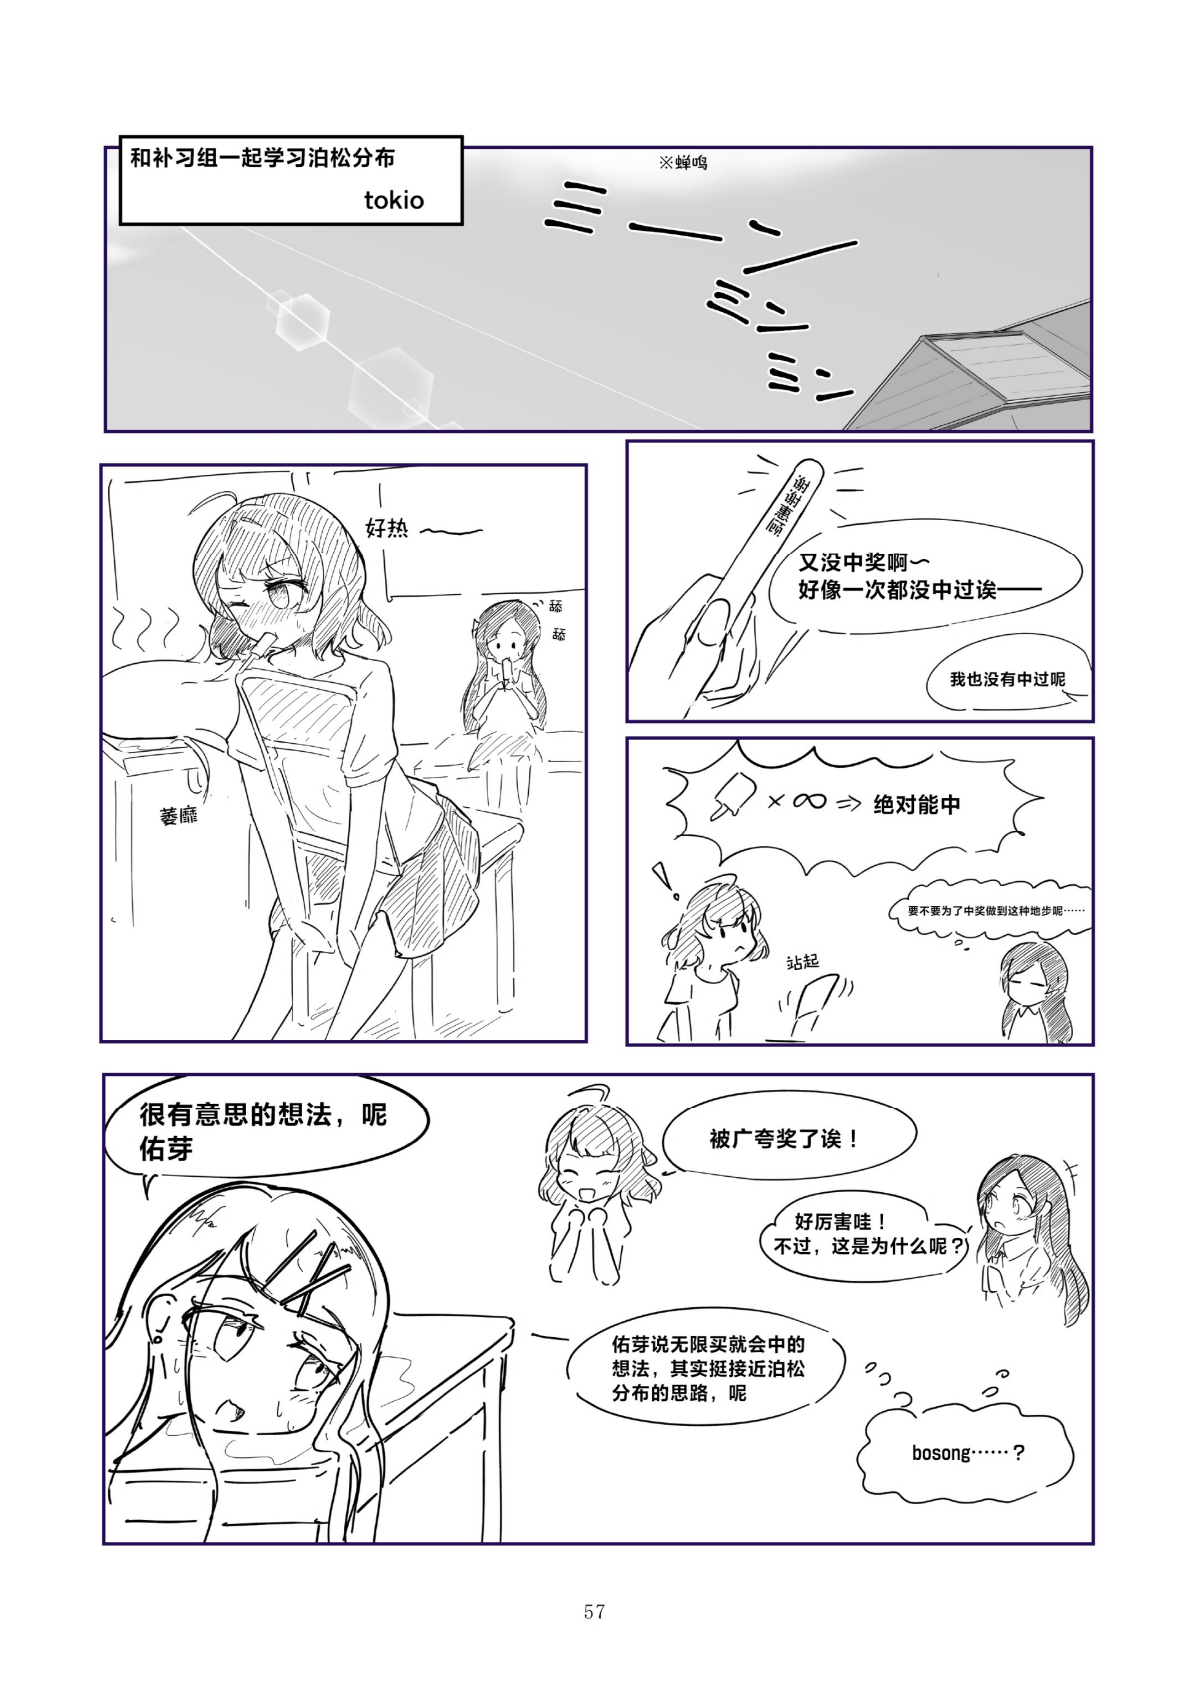
\includegraphics[width=0.96\textwidth]{figures/extracted/ml-optimization-seminar-1/poisson-distribution-page-01.png}

{\small 和补习组一起学习泊松分布，第 1 页\par}
\end{figure}
\begin{figure}[p]
\centering
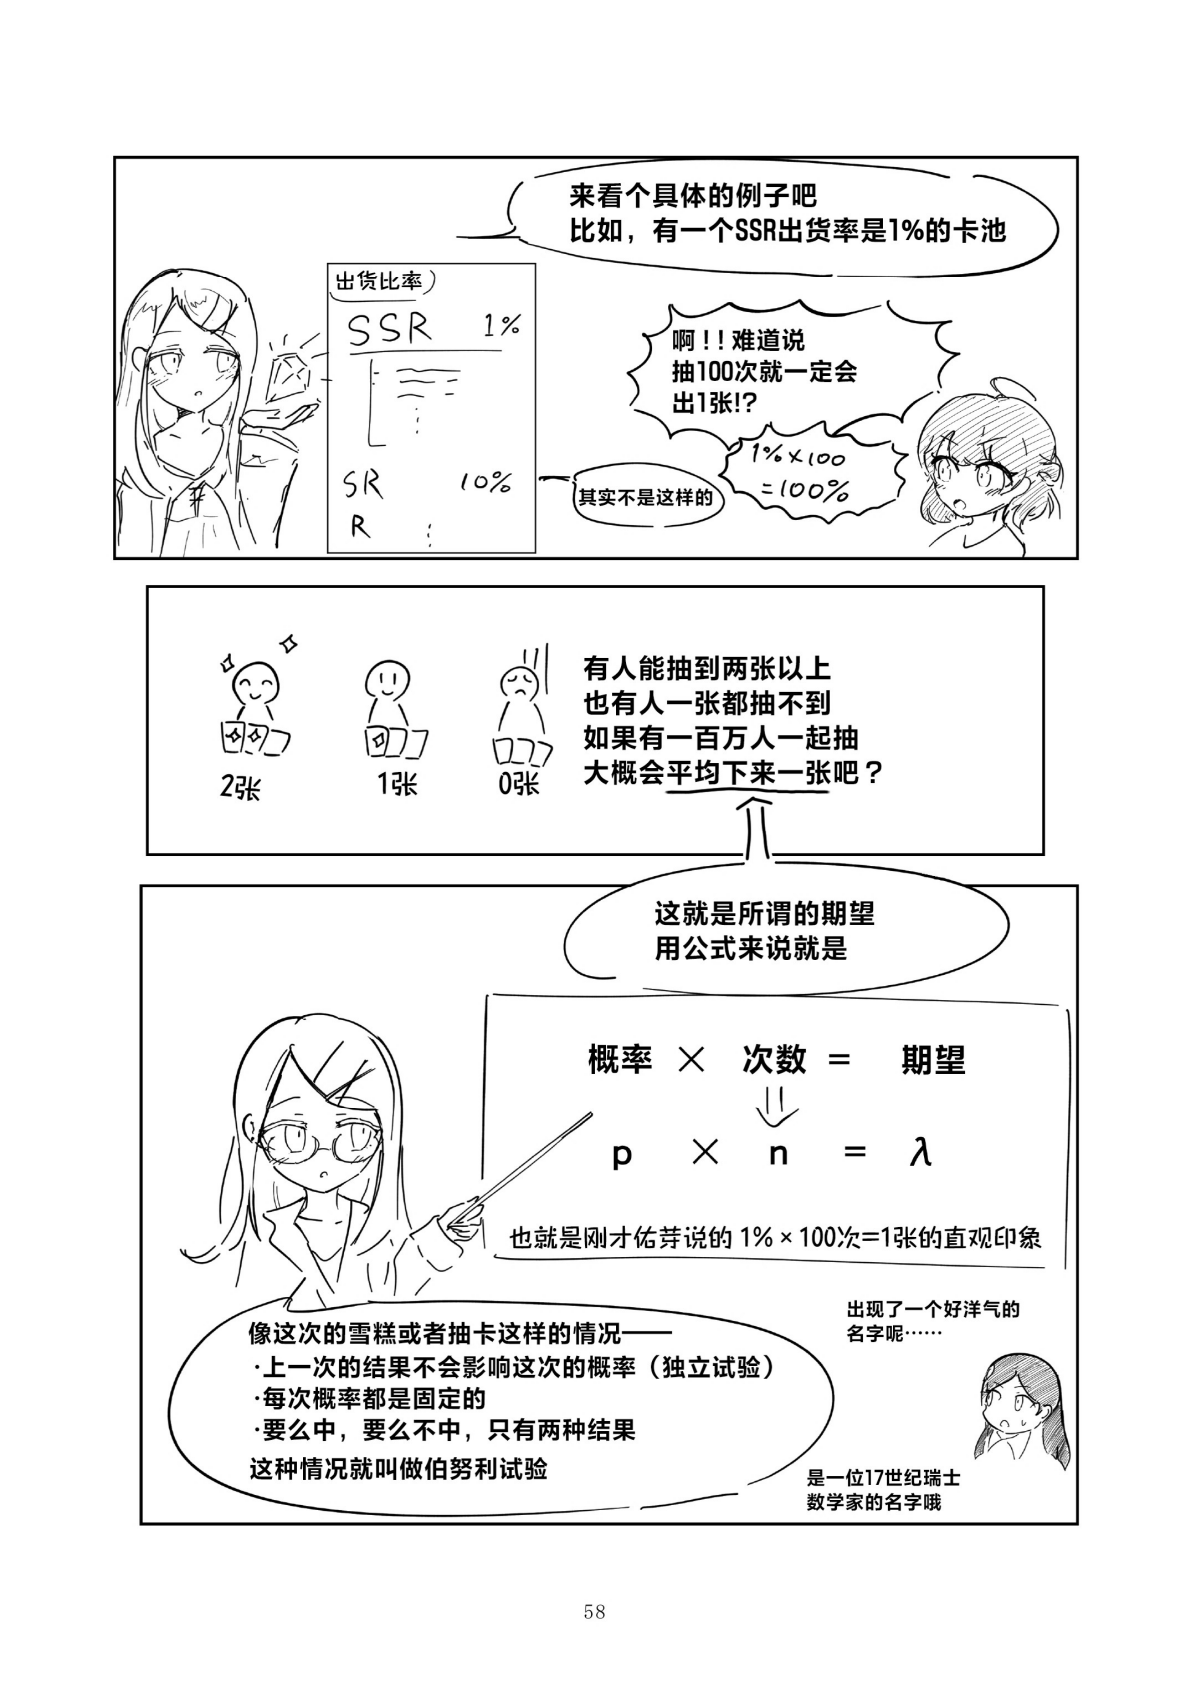
\includegraphics[width=0.96\textwidth]{figures/extracted/ml-optimization-seminar-1/poisson-distribution-page-02.png}

{\small 和补习组一起学习泊松分布，第 2 页\par}
\end{figure}
\begin{figure}[p]
\centering
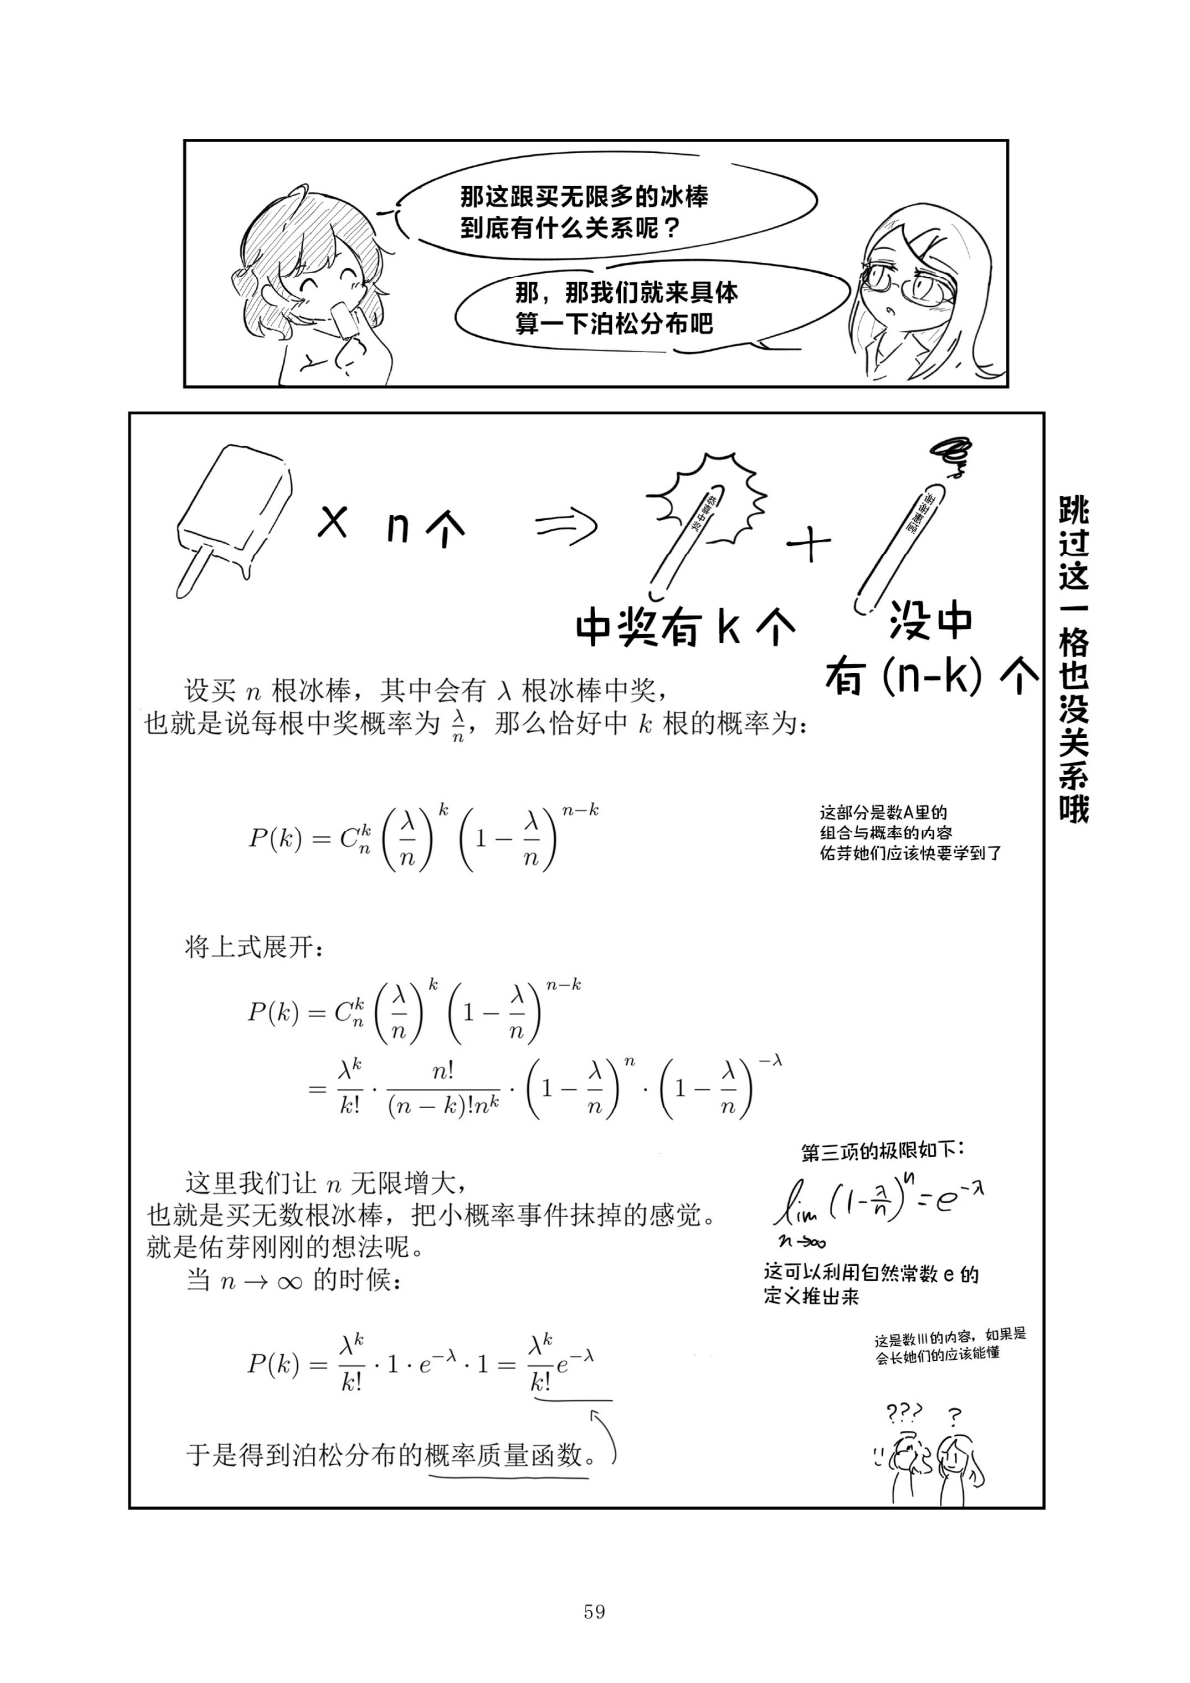
\includegraphics[width=0.96\textwidth]{figures/extracted/ml-optimization-seminar-1/poisson-distribution-page-03.png}

{\small 和补习组一起学习泊松分布，第 3 页\par}
\end{figure}
\begin{figure}[p]
\centering
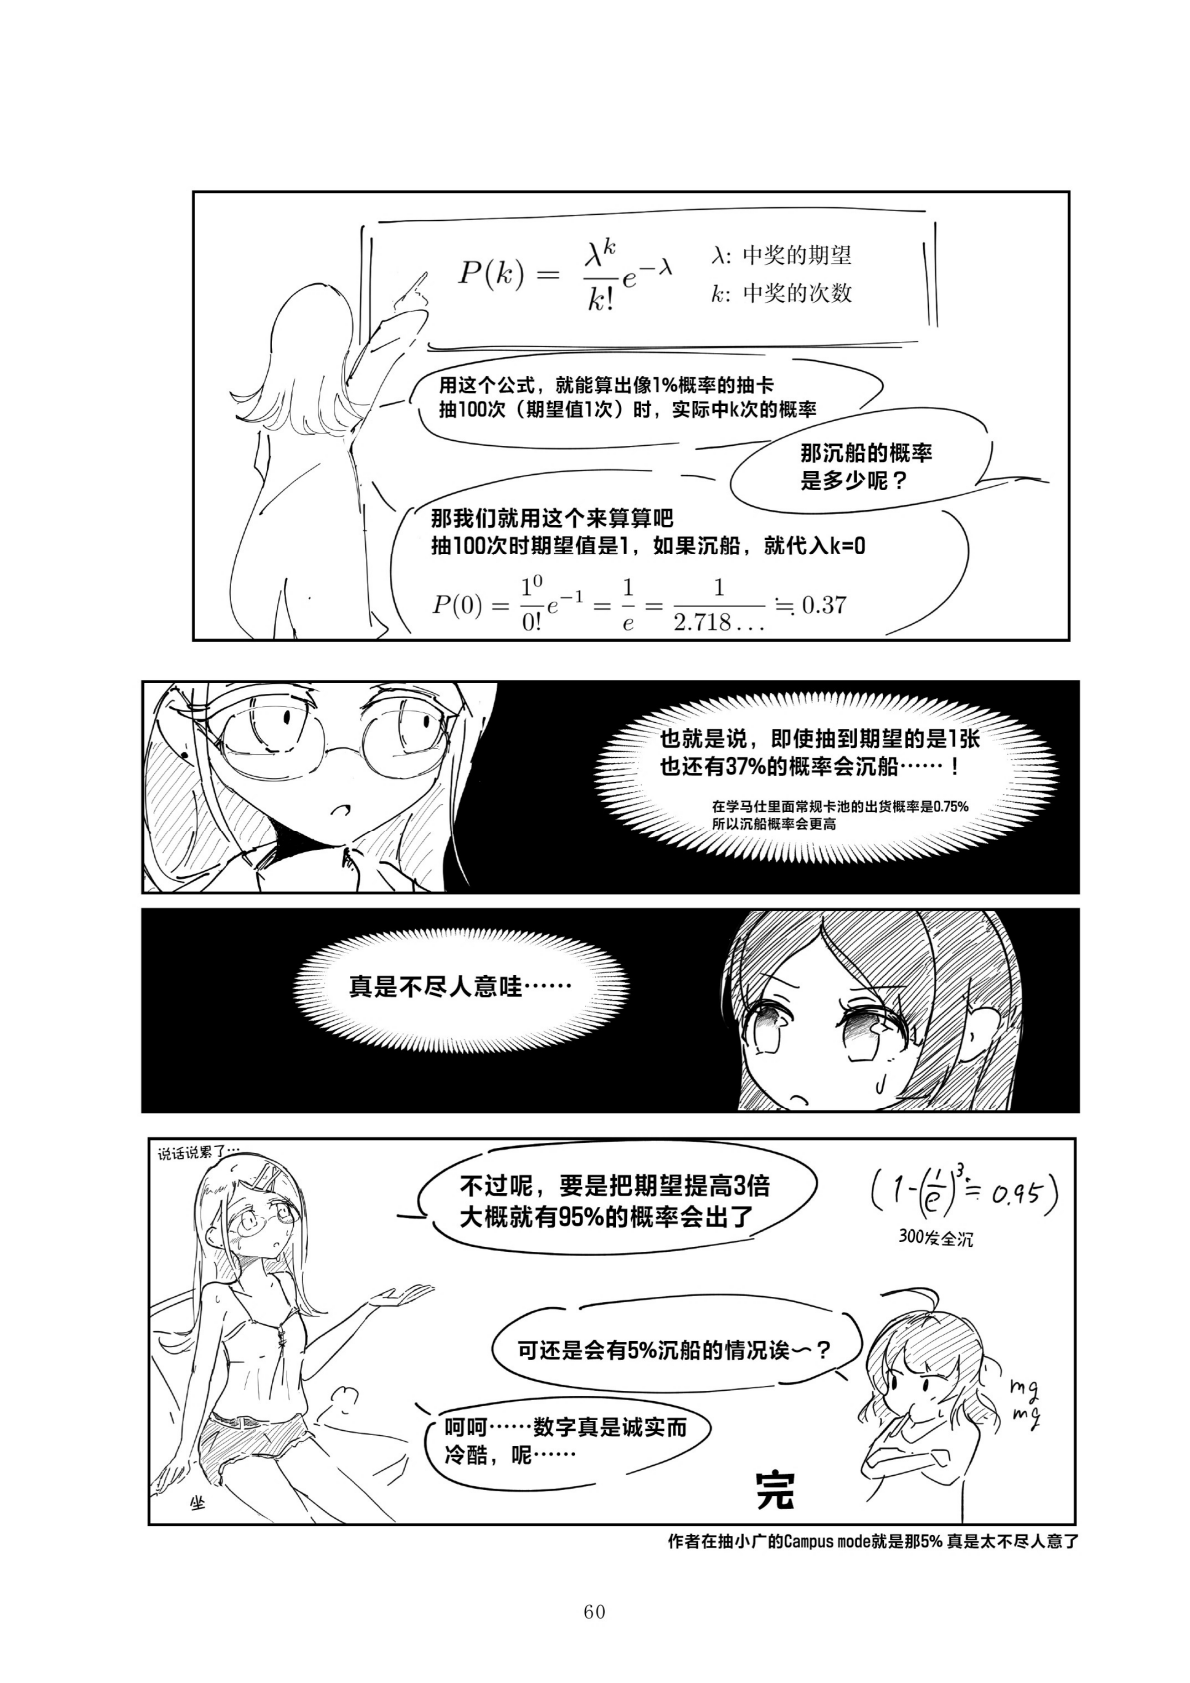
\includegraphics[width=0.96\textwidth]{figures/extracted/ml-optimization-seminar-1/poisson-distribution-page-04.png}

{\small 和补习组一起学习泊松分布，第 4 页\par}
\end{figure}
\clearpage
\section*{主催后记}
\addcontentsline{toc}{section}{主催后记}
\begin{figure}[p]\centering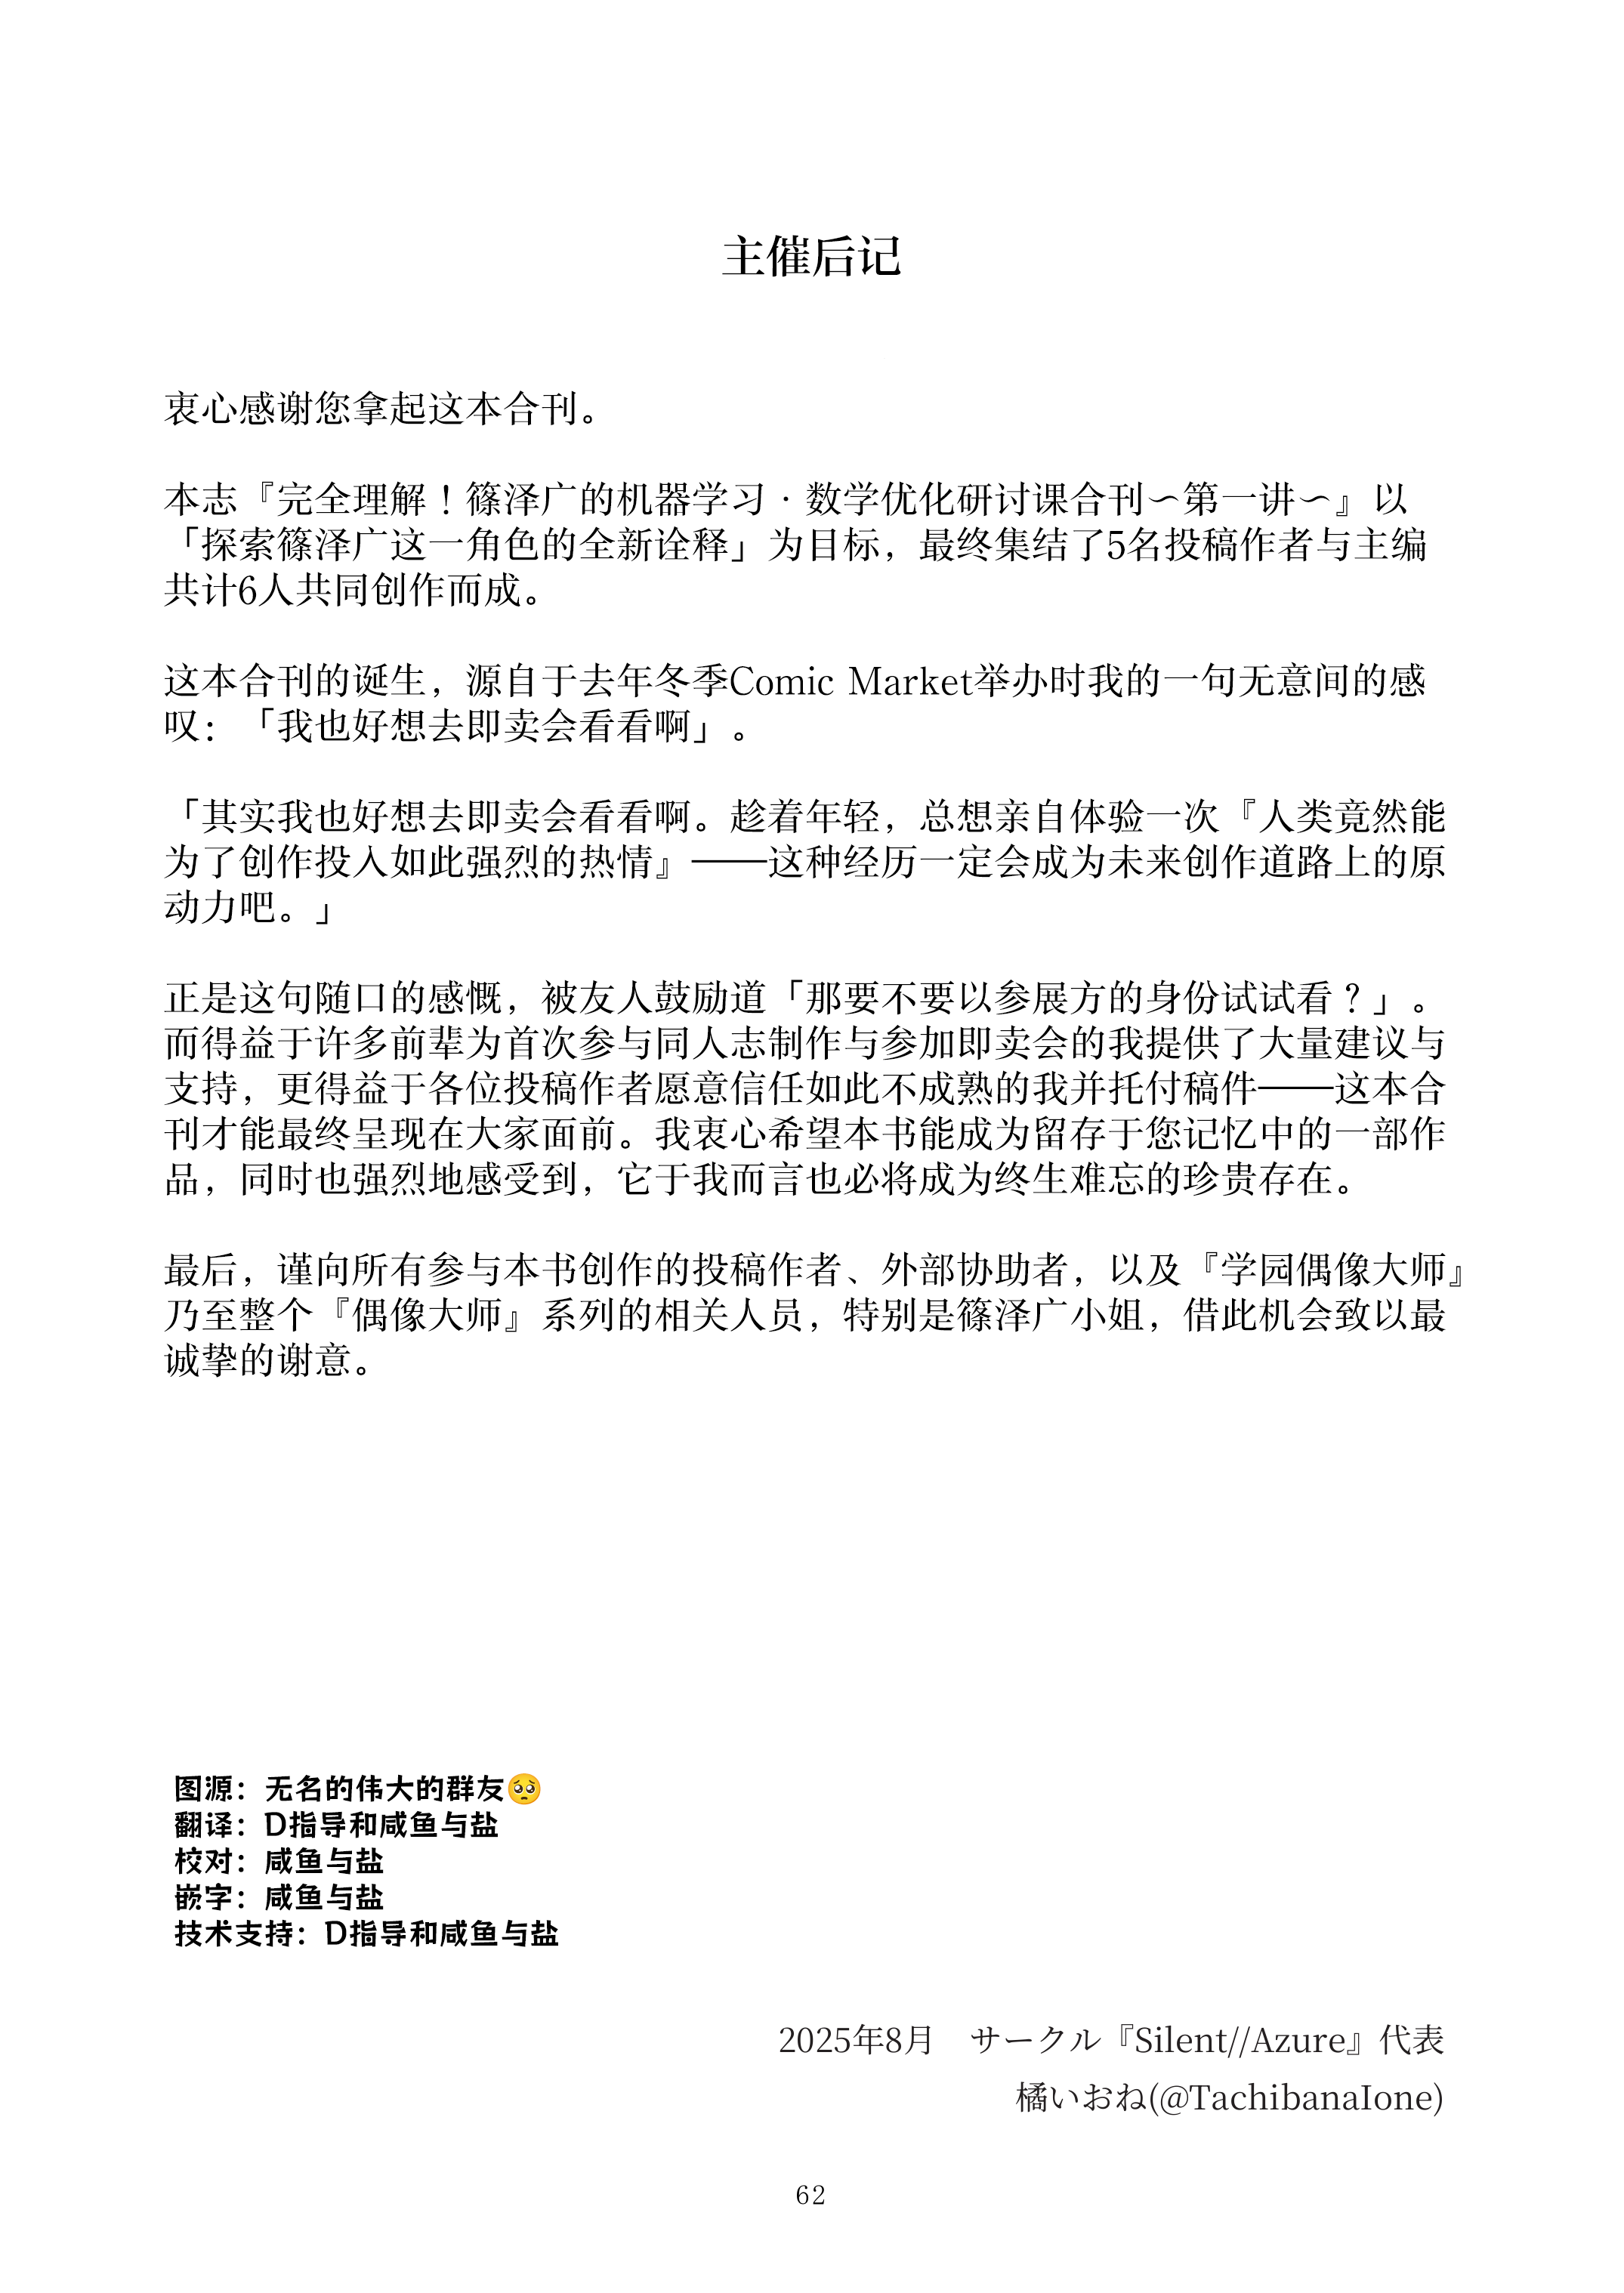
\includegraphics[width=0.96\textwidth]{figures/extracted/ml-optimization-seminar-1/organizer-afterword.png}\end{figure}
\clearpage
\section*{投稿者后记}
\addcontentsline{toc}{section}{投稿者后记}
\begin{figure}[p]\centering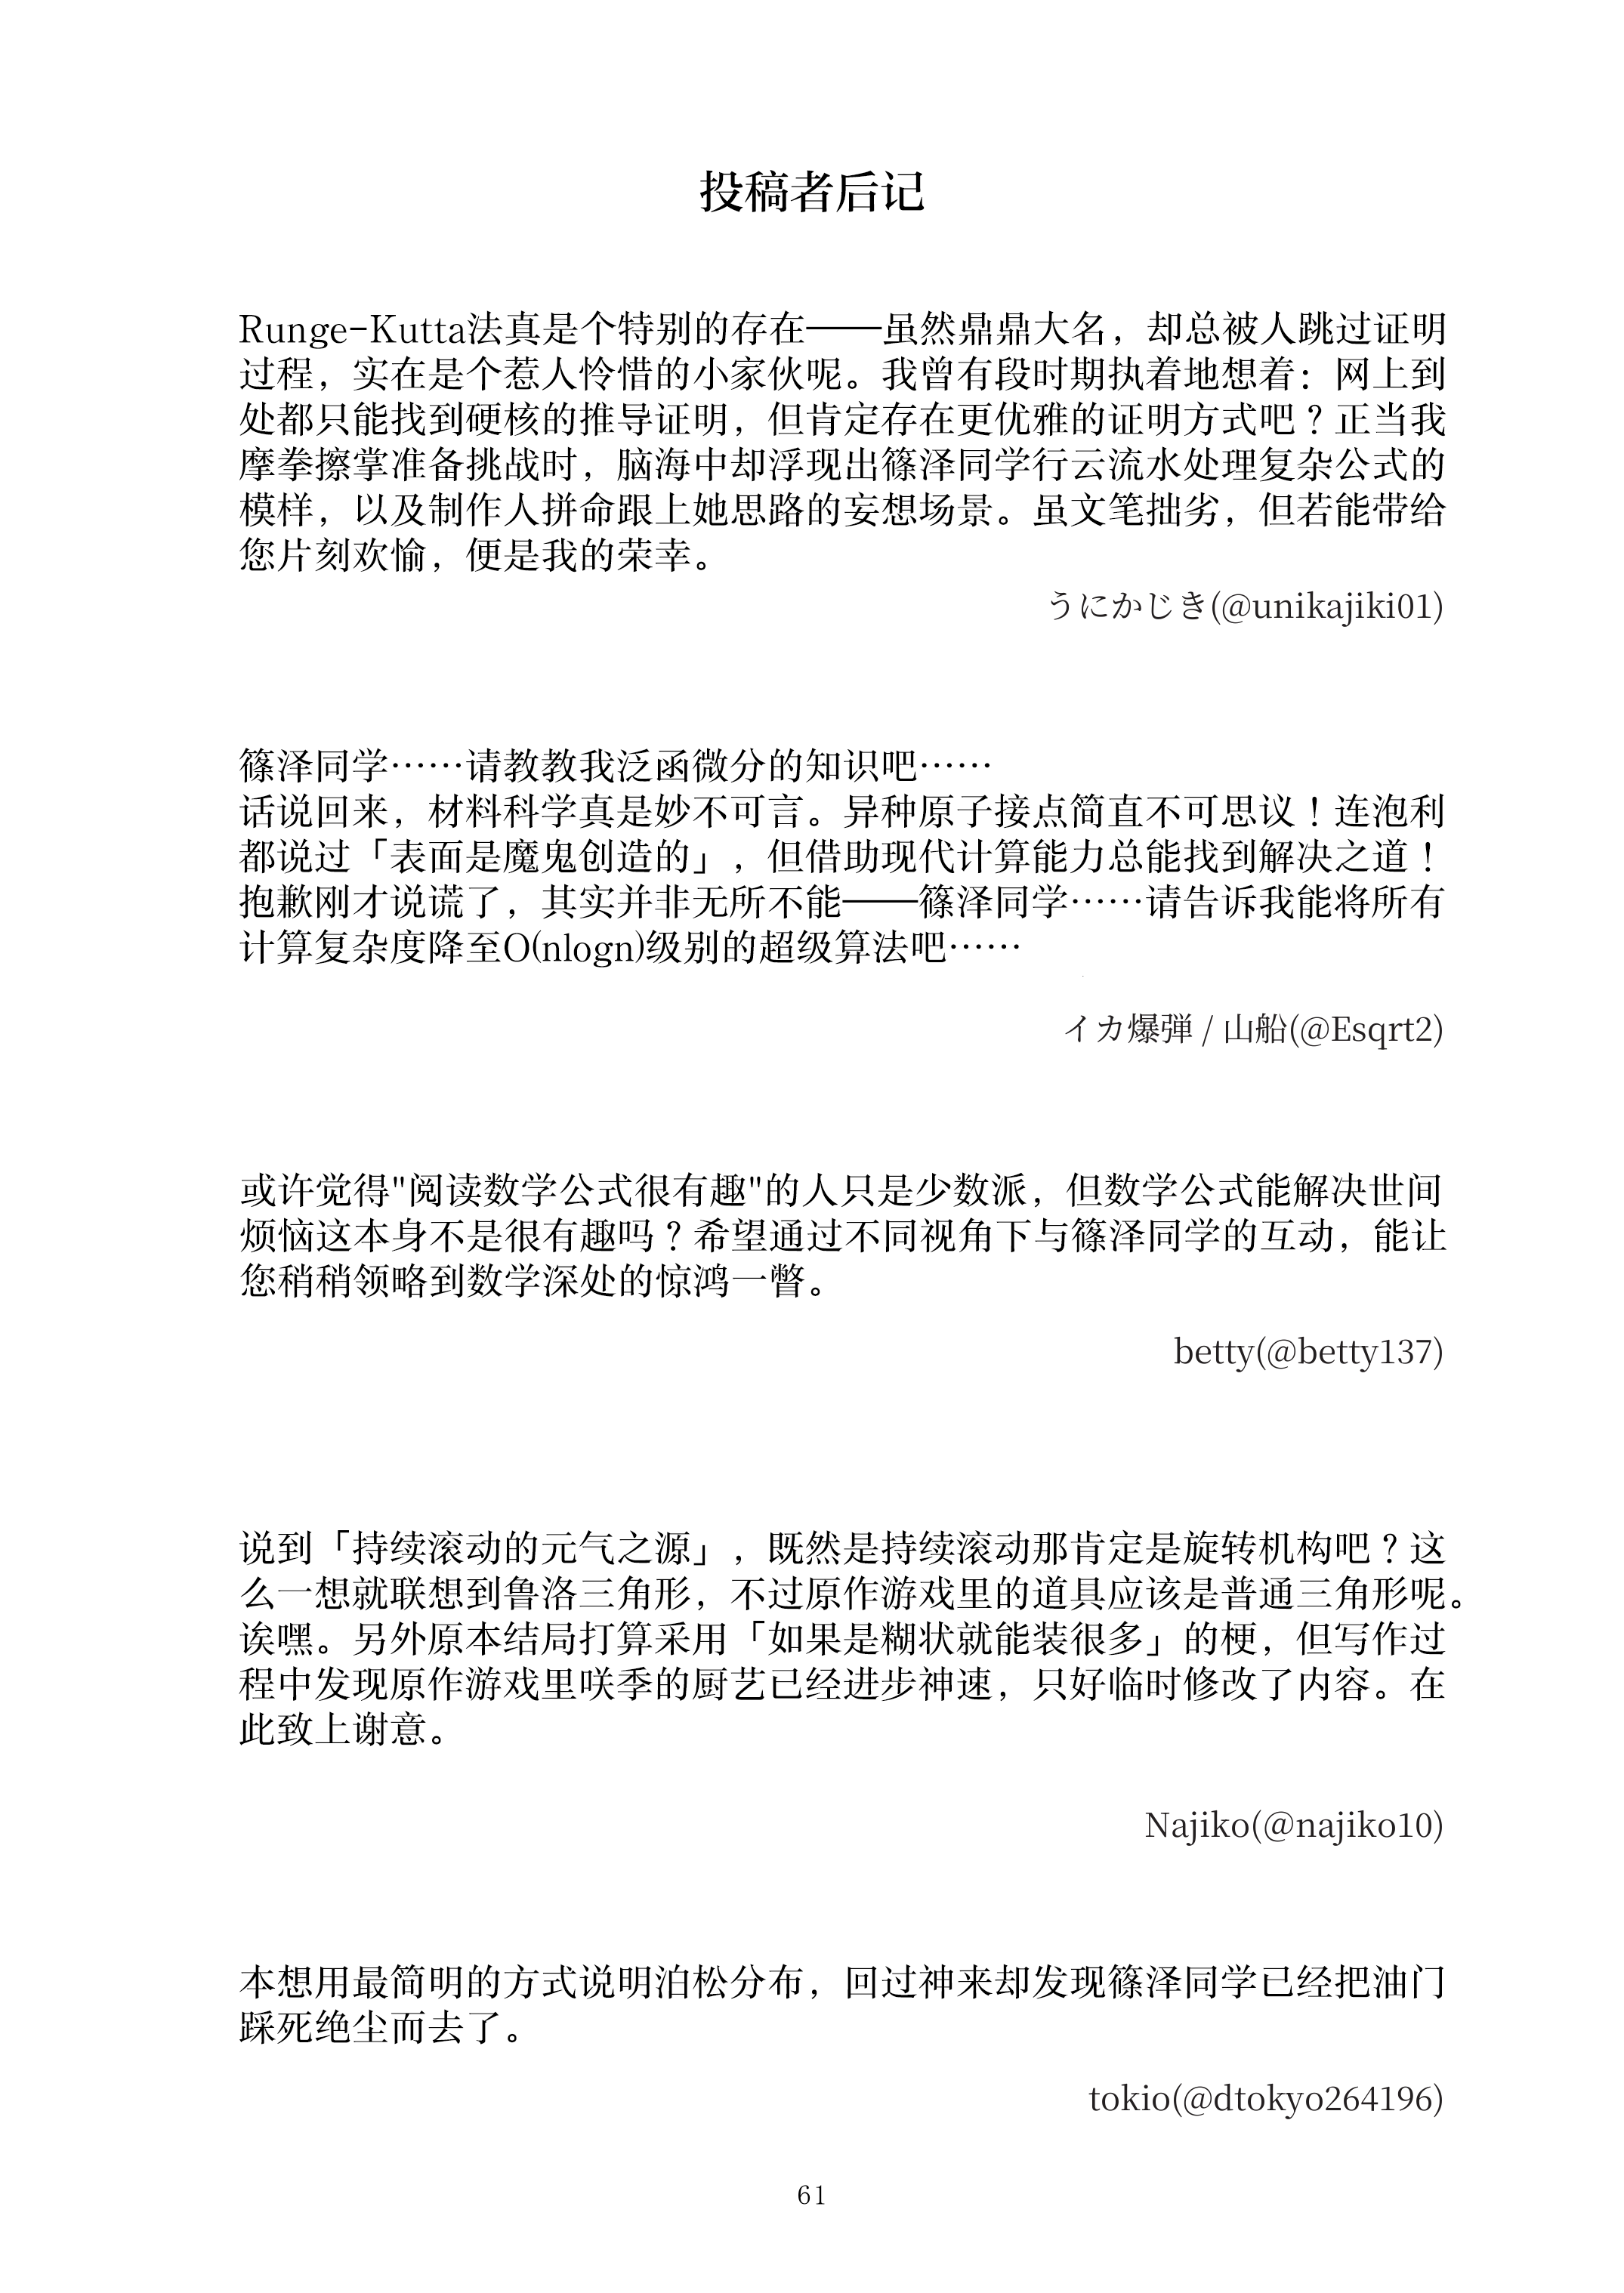
\includegraphics[width=0.96\textwidth]{figures/extracted/ml-optimization-seminar-1/contributor-afterword.png}\end{figure}
